\chapter{Topological quantum computation}
\label{Chap:TQC}
In this chapter, we explain how to perform topological fault-tolerant quantum computation on the surface code.
All operations employed are nearest-neighbor (at most) two-qubit gates and signle-qubit measurements on a 2D array of qubits.
This property is quite favorable for the fabrication of qubits and their control lines on a chip.
Fault-tolerance ensures that no local noise during any sort of operations ever spoil the quantum computation, if the noise strength is smaller than a certain threshold value, as seen below.

We first introduce the defect pair qubit, a logical qubit using a pair of defects on the surface, which allows us to encode many logical qubits on the surface.
Then, we explain the elementary operations of defects by local quantum information processing.
A braiding operation, based on the elementary operations, of the defects is further utilized to implement the logical CNOT gate between the defect pair qubits.
Combining with the topologically protected operations, the magic states are injected 
and distilled for fault-tolerant universal quantum computation.
Based on these understandings, we introduce a topological diagram and the topological calculus on it, as a set of the transformations that preserve the logical actions on the code space.
These provide us with a deep understanding of topological quantum computation on the surface. 
Finally, we return to the microscopic viewpoint to explain how topological quantum error correction is executed and analyzed.


\section{Defect pair qubits}
\label{Sec:DPQ}
In order to perform quantum computation of $N$ qubits, we have to arrange $N$ logical qubits in the code subspace while keeping their code distance long enough.
A way of doing this is to use a surface of higher genus. 
Specifically, we use a large planar surface and punch holes on it, which we call defects on the surface.

In Sec.~\ref{subsec:planar}, we have seen that we can define a logical qubit by introducing a defect on a planar surface, where the stabilizer generators inside the defect region 
are removed from the stabilizer group.
The logical operators are defined by a nontrivial cycle surrounding the defect and a chain connecting the defect to the boundary.
If we introduced many degrees of freedom, i.e., many defects
based on this strategy, the logical operators defined by chains connecting each defect to the boundary would become complicated.
To avoid this, we use a pair of defects to define a logical qubit, which we call a {\it defect pair qubit}\index{defect pair qubit}.

\begin{figure}[t]
\centering
%\sidecaption
% Use the relevant command for your figure-insertion program
% to insert the figure file.
% For example, with the option graphics use
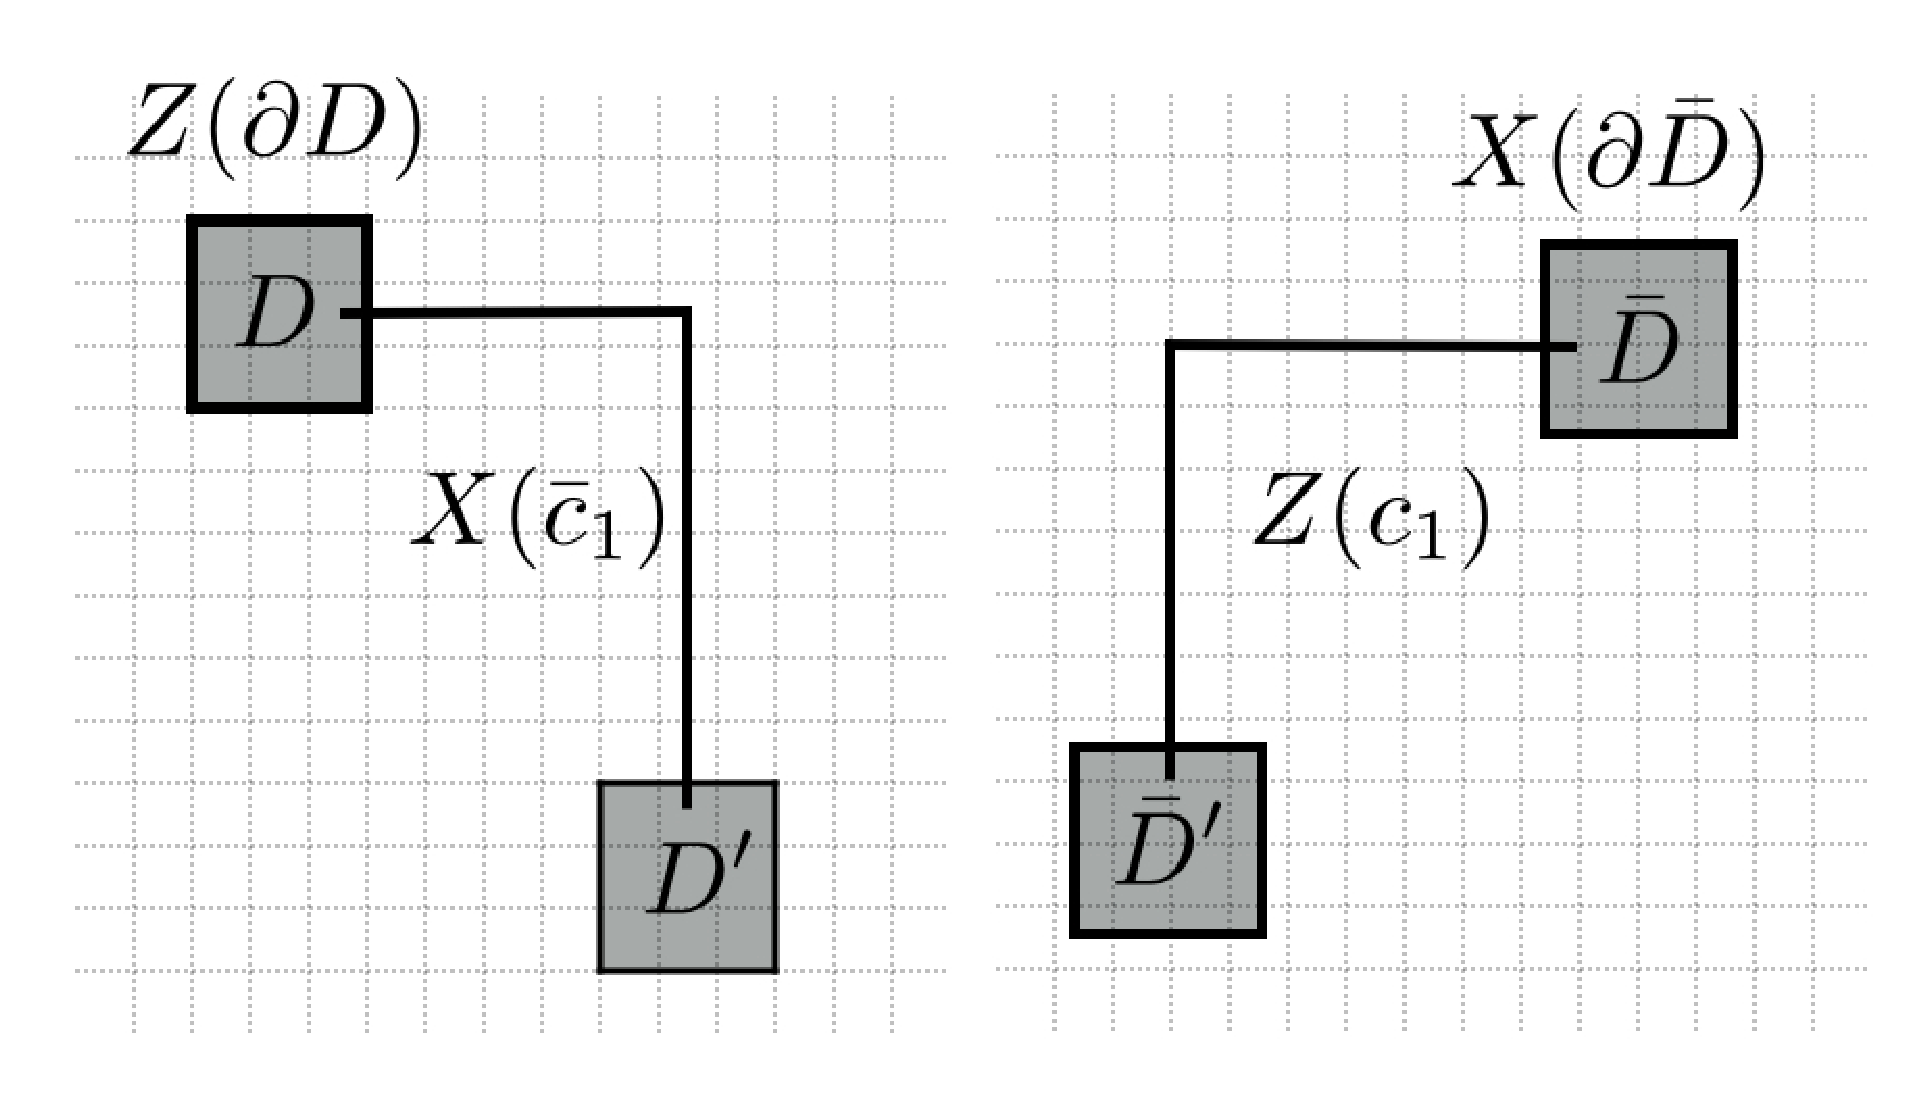
\includegraphics[width=120mm]{fig73.eps}
%
% If not, use
%\picplace{5cm}{2cm} % Give the correct figure height and width in cm
%
\caption{Primal (left) and dual (right) defect pair qubits. 
The primal defect pair qubit is defined by removing the plaquette operators inside the defect regions $D$ and $D'$. 
Then the cycle $\partial D$ around the defect becomes a nontrivial cycle, by which the logical $Z$ operator $Z(\partial D)$ is defined. 
The logical $X$ operator $X(\bar c_1)$ is defined as a dual 1-chain $\bar c_1$ connecting two defects. 
Any homologically equivalent logical operators acts the same way on the code space.
The dual defect pair is defined similarly, but the basis is changed by the Hadamard transformation.
  }
\label{fig73}       % Give a unique label
\end{figure}
We define two defect regions $D \in C_2$ and $D'\in C_2$, as shown in Fig.~\ref{fig73}.
We remove all $Z$-type stabilizer generators inside these regions, i.e., $\{ A_m\} _{f_m \in D \cup D'}$.
Thus, the operators $Z(\partial D)$ and $Z(\partial \bar D')$ are not stabilizer operators.
Instead, we append a $Z$-type stabilizer operator $Z(\partial D+\partial \bar D)$ as a stabilizer generator.
Moreover, we also append the Pauli $X$ operator on all edge qubits inside (not including the boundary) the regions $D \cup D'$, i.e., 
$\{ X_l \}_{e_l \in (D \cup D') \backslash (\partial D \cup \partial D')}$.
By this definition, the star ($X$-type) stabilizer generators in the defect region are still in the stabilizer group. 
We choose $Z(\partial D)$ as a logical operator, because it commutes with all stabilizer operators, but does not belong to the stabilizer group.
Because $Z(\partial D + \partial \bar D)$ is a stabilizer operator, $Z(\partial D')$ also acts the same way, i.e., $Z(\partial D) \sim Z(\partial D')$.
Moreover, 
the actions of operators represented by 
the homologically equivalent cycles are the same.
The logical $X$ operator is given by $X(\bar c_1)$, with a dual 1-chain $\bar c_1$ connecting two defects, as shown in Fig.~\ref{fig73}.
The actions of the operators represented by any homologically equivalent chains in the sense of relative homology are the same.
That is, we may choose any dual 1-chain $\bar c_1$
which connects two defect regions $D$ and $D'$.
The code distance is given by the circumference of the defect or the distance between two defects.
Because the plaquette operators on the primal lattice are removed, we call these defects and the logical qubit {\it primal defects} and {\it primal defect pair qubit}, respectively.

Similarly, we can also define a logical qubit by removing the star ($X$-type) stabilizer operators on the dual defect regions $\bar D$ and $\bar D'$ defined on the dual lattice as shown in Fig.~\ref{fig74}.
We call such defects and the logical qubit {\it dual defects} and {\it dual defect pair qubit}, respectively.
Hereafter, the planar surface code state, on which the defects are introduced, is referred to as {\it vacuum}.
Below we will explain how defect qubits are created, deformed, and moved in the vacuum. 

\section{Defect creation, annihilation, and movement}
\index{defect creation, annihilation, and movement}
\label{Sec:DefectOperation}
\begin{figure}[t]
\centering
%\sidecaption
% Use the relevant command for your figure-insertion program
% to insert the figure file.
% For example, with the option graphics use
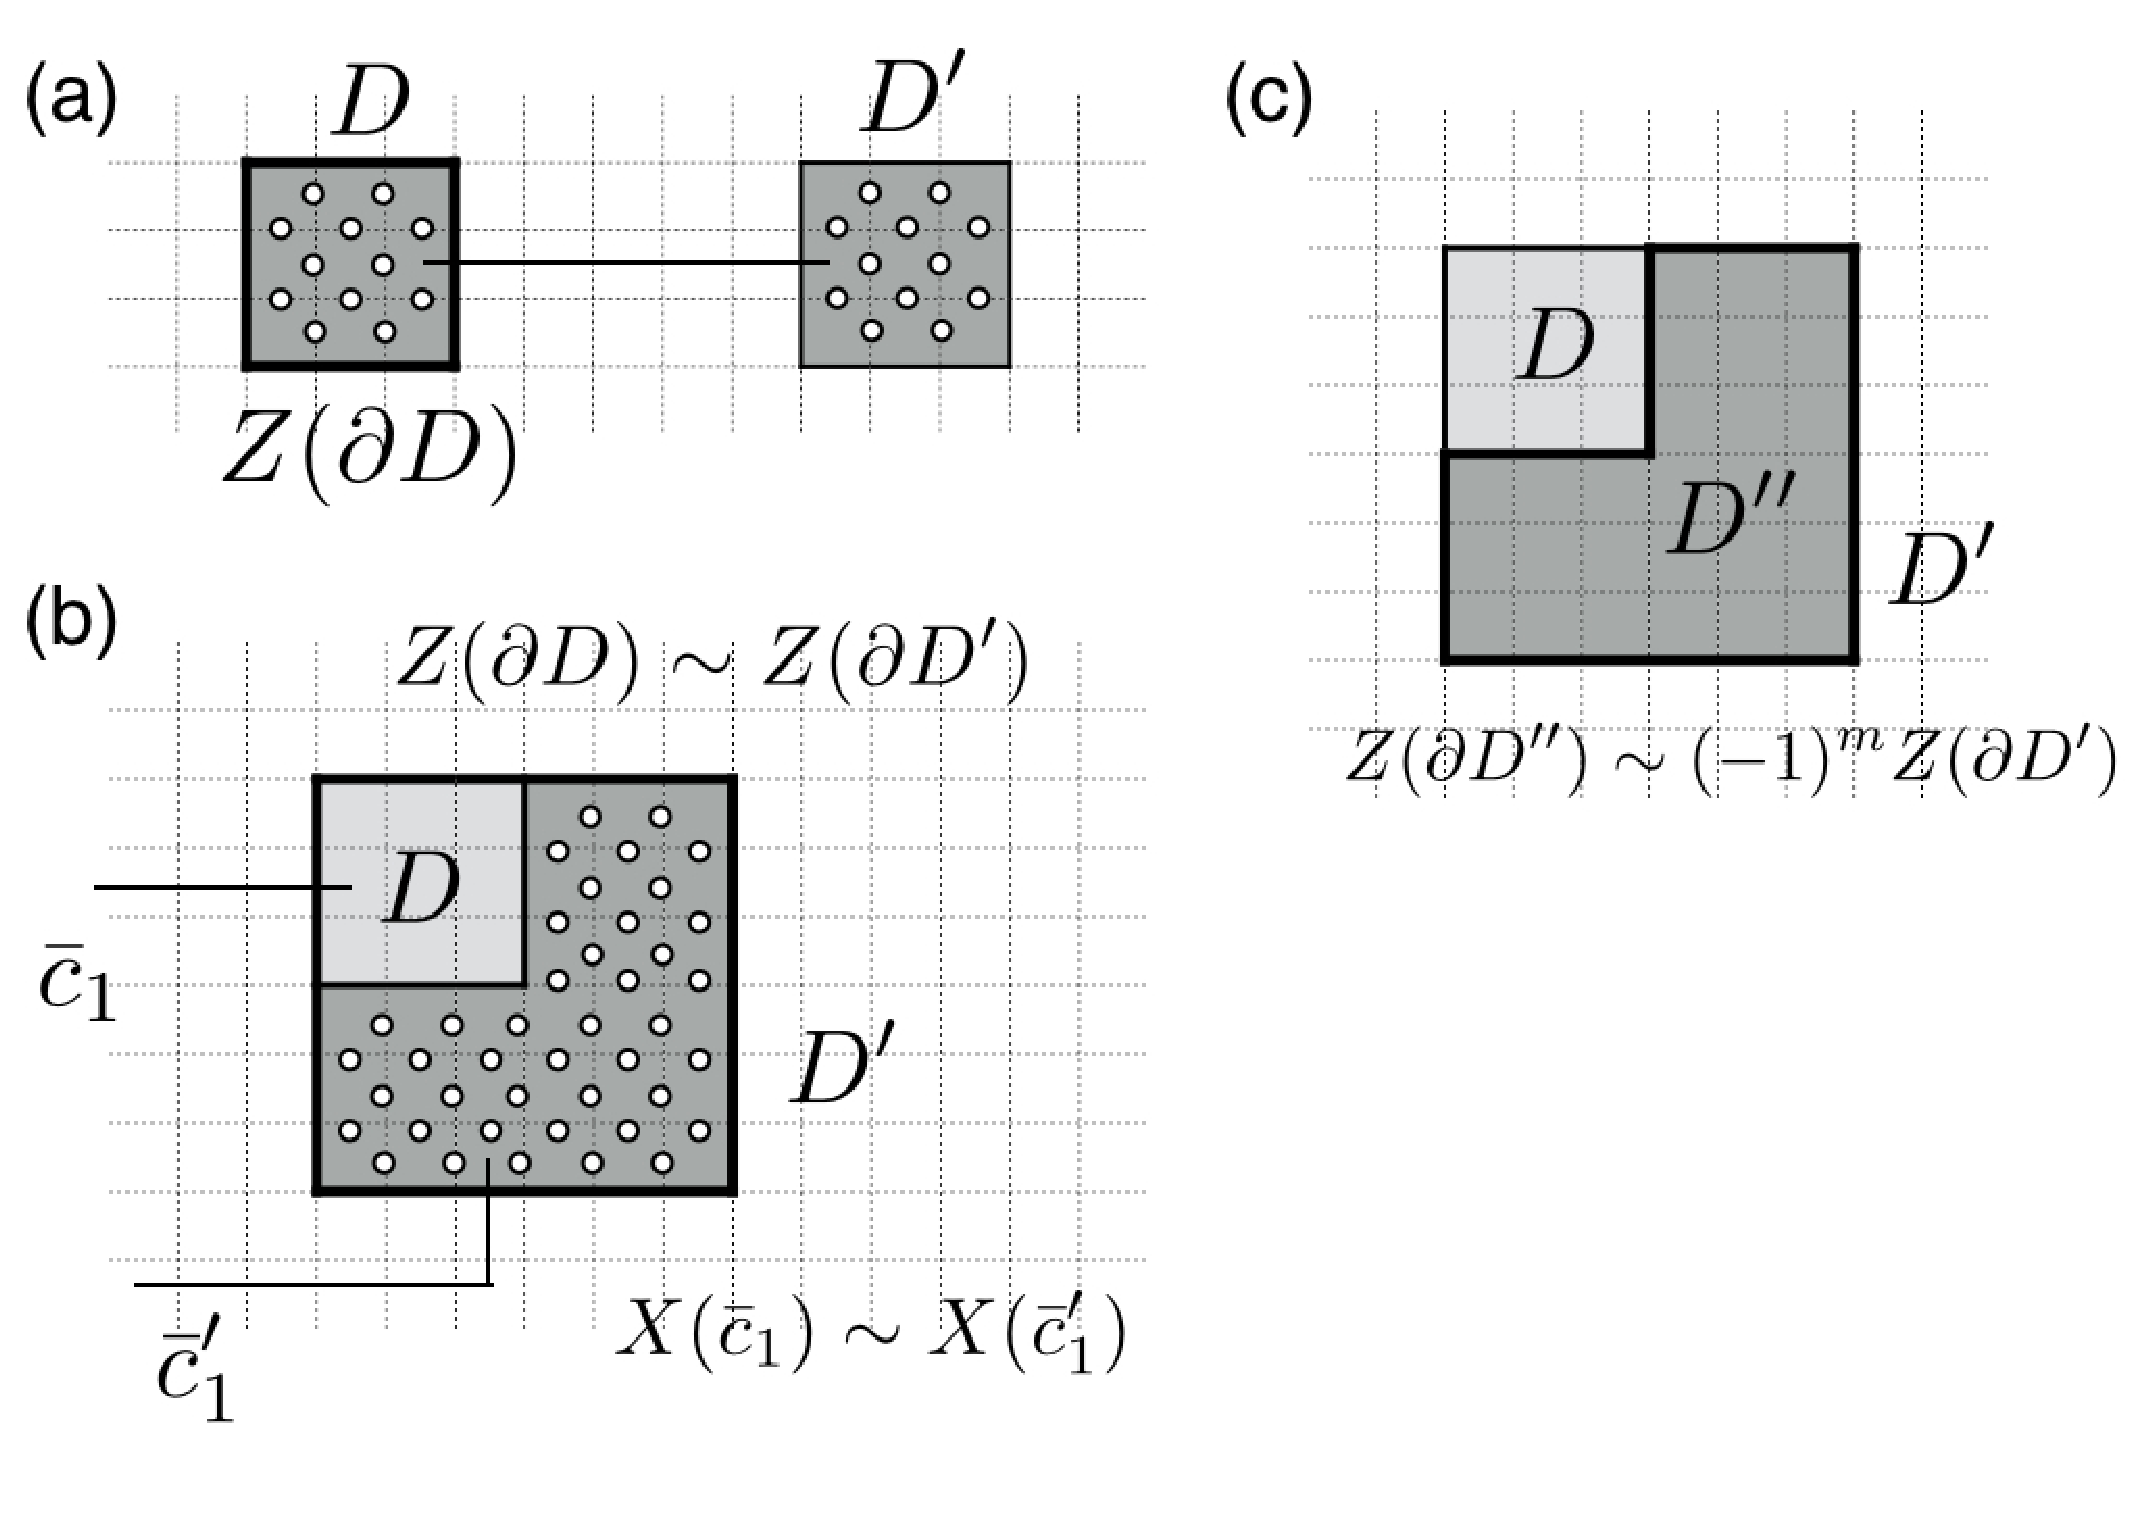
\includegraphics[width=130mm]{fig74.eps}
%
% If not, use
%\picplace{5cm}{2cm} % Give the correct figure height and width in cm
%
\caption{(a) A defect creation. 
The qubits inside the defect regions (excluding the qubits on the boundary), denoted by circles, are measured in the $X$-basis. 
(b) The defect region $D$ is expanded into $D'$ by measuring the qubits inside the region $D'$ in the $X$-basis, where the encoded quantum information is preserved. 
(c) A defect region $D'$ is contracted into $D$ by measuring the plaquette operators in $D'' = D' \backslash D$. 
The logical operator $Z$ after the contraction is defined depending on the measurement outcome $m$. }
\label{fig74}       % Give a unique label
\end{figure}
The defect creation is accomplished by measuring the qubits inside the defect region $D$, not including the qubits on its boundary, in the $X$-basis [see Fig.~\ref{fig74} (a)].
These measurements remove the plaquette operators inside $D$ from the stabilizer group, because these $X$-basis measurements do not commute with them.
On the other hand, the measurements do commute with the star operators, and hence a parity of four measurement outcomes corresponding to a star operator is always even (if there is no measurement error).
While the measurement outcomes are random, we can prepare all measured qubits to be in the $|+\rangle$ state by applying $Z$ operators according to the measurement outcomes.
(In practice, there is no need to apply the $Z$ operations. 
It is enough to keep the information of the byproduct Pauli operator dependent on the measurement outcomes.)

As the qubits on the boundary are not measured, the post-measurement state is stabilized by $Z(\partial D)$.
In order to create a pair of defects, we do the same thing for another defect $D'$.
Apparently, the resultant state is stabilized by $Z(\partial D + \partial D')$ and satisfies the definition of the defect pair qubit. 
Moreover, the logical qubit is stabilized by $Z(\partial D)$ and hence a logical $Z$-basis state is prepared.

The defect region can be expanded by creating a larger defect $D'$, which includes the original defect region $D$, i.e., $D \subset D'$, 
as shown in Fig.~\ref{fig74} (b).
We can choose $Z(\partial D')$ as a logical $Z$ operator of the defect pair qubit, so that the information with respect to $Z(\partial D')$ is preserved during this operation.
(Recall that logical operators act the same if the corresponding cycles are homologically equivalent. Thus we can choose a large enough cycle 
surrounding the defect in advance.)
We can expand the defect region step-by-step such that, at each step, a logical $X$ operator is untouched as shown in Fig.~\ref{fig74} (b).
(Or equivalently, we can compensate for the difference in the logical $X$ operator according the $X$-basis measurement outcomes inside the defect region.)
Thus, the information with respect to the logical $X$ operator is also preserved.
Accordingly, the logical information of the defect pair qubit is stored, but now the defect region $D$ is expanded into $D+D'$.

The defect annihilation is executed by measuring the plaquette operators inside the region $D$ to restore them to the stabilizer group.
The surface with a defect $D$ is rewritten by
\begin{eqnarray}
|D\rangle \propto \prod _{e_l \in D} \left(\frac{I+X_{l}}{2} \right) |v\rangle,
\end{eqnarray}
where $|v\rangle$ indicates the surface code state without defect, i.e., vacuum.
Thus, $|D\rangle$ is a superposition of all possible applications of $X$ operators on the vacuum $|v\rangle$.
The measurements of the plaquette operators collapse the superposition.
By applying a recovery operation inside the region $D$ such that all eigenvalues becomes $+1$, the defect is annihilated.
(Note that there is no need to actually apply the recovery operation. It is enough to keep the record of the eigenvalues.)
The parity of all measurement outcomes of the plaquette operators inside $D$ corresponds to the eigenvalue of $Z(\partial D)$, because we have 
\begin{eqnarray}
Z(\partial D) = \prod _{f_m \in D} Z(\partial f_m)= \prod _{f_m \in D} A_m.
\end{eqnarray}
This indicates that a logical $Z$-basis measurement can be done by annihilating the defect completely.

Suppose a defect region $D$ inside the defect region $D'$ (i.e., $D \in D'$) is annihilated by measuring the qubits inside $D$, as shown in Fig.~\ref{fig74} (c).
We can then obtain the eigenvalue $(-1)^m$ ($m=0,1$) of $ Z (\partial D)$.
Let $D''$ be the complement of $D$ in $D'$.
Because we have 
\begin{eqnarray}
Z( \partial D')  = Z(\partial D'' ) Z( \partial D),
\end{eqnarray}
depending on the eigenvalue $(-1)^m$, the operator $(-1)^{m }Z(\partial D'')$ acts as the logical operator of the defect $D''$.
Thus, the defect $D'$, consisting of the defect pair qubit, is contracted into $D''$ without changing the stored quantum information (up to the logical Pauli $X$ flip).

\begin{figure}[t]
\centering
%\sidecaption
% Use the relevant command for your figure-insertion program
% to insert the figure file.
% For example, with the option graphics use
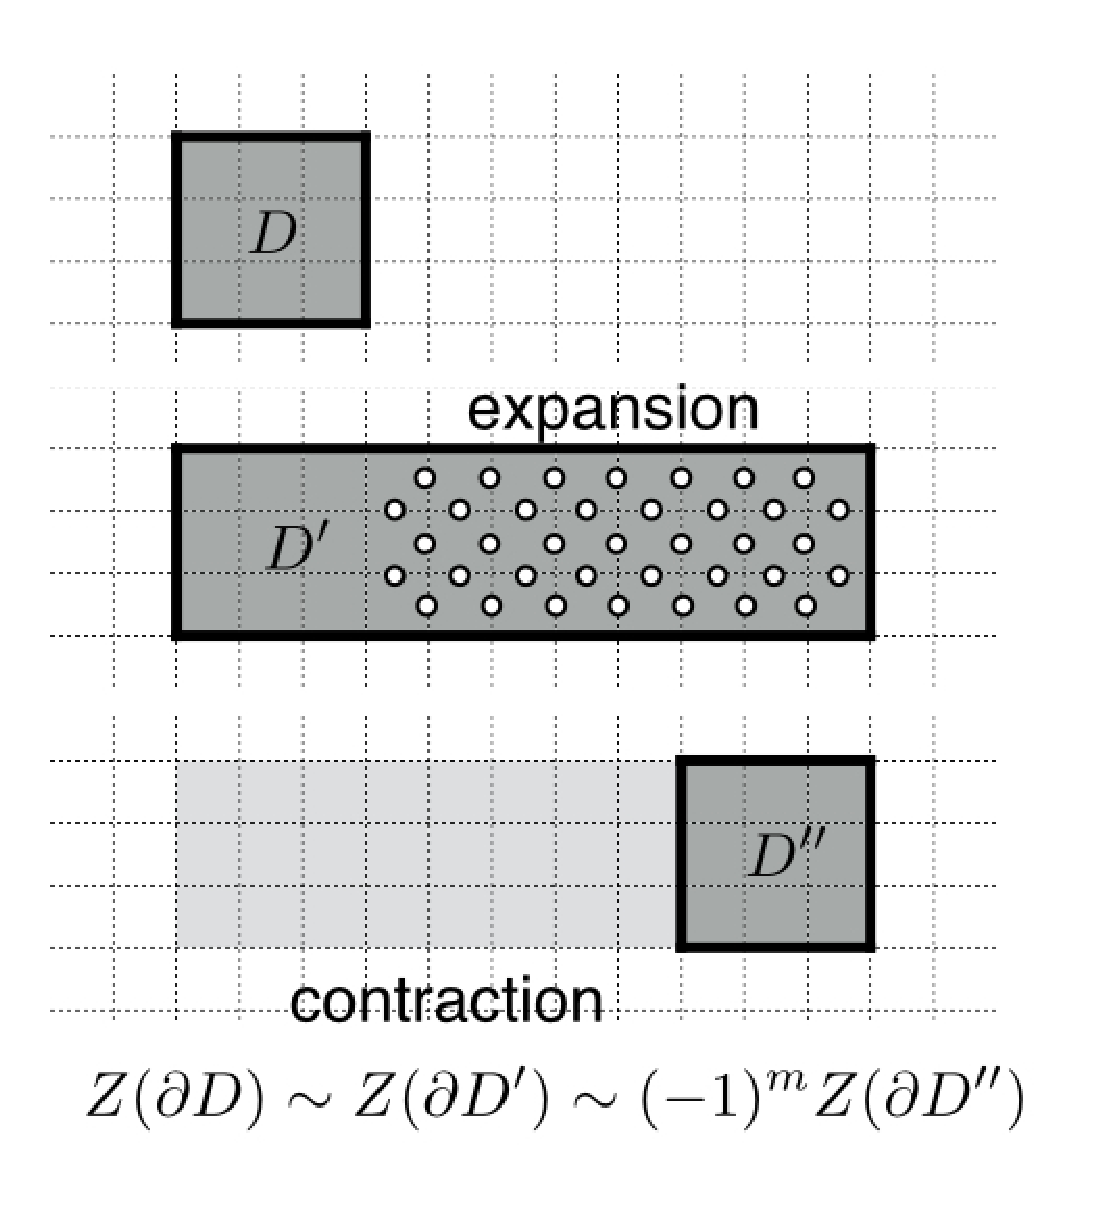
\includegraphics[width=100mm]{fig78.eps}
%
% If not, use
%\picplace{5cm}{2cm} % Give the correct figure height and width in cm
%
\caption{A defect movement by expansion and contraction.}
\label{fig78}       % Give a unique label
\end{figure}
The defect movement on the surface is implemented by combining the defect expansion and contraction, as shown in Fig.~\ref{fig78}.
At first, we expand a defect $D$ into $D'$ ($D \in D'$) by the previously mentioned procedure.
Second, the defect region $D$ is annihilated, and we obtain the eigenvalue $(-1)^m$ of $ Z (\partial D)$.
As we already pointed out, the stored logical information is unchanged under these procedures up to the logical Pauli $X$ operator depending on the measurement outcome $m$.

\begin{figure}[t]
\centering
%\sidecaption
% Use the relevant command for your figure-insertion program
% to insert the figure file.
% For example, with the option graphics use
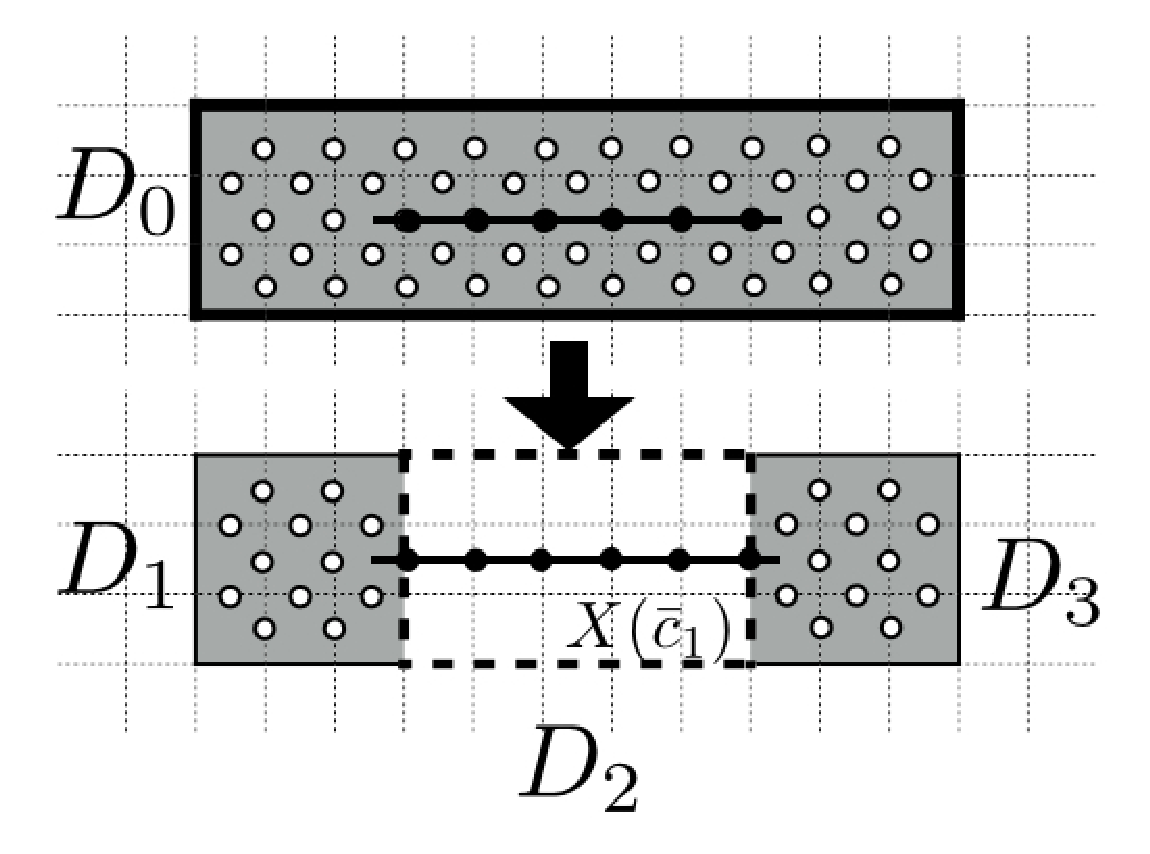
\includegraphics[width=100mm]{fig79.eps}
%
% If not, use
%\picplace{5cm}{2cm} % Give the correct figure height and width in cm
%
\caption{A preparation of the logical $X$-basis state by creation of a defect region $D_0$ and annihilation of a defect region $D_2$ between two defect regions $D_1$ and $D_3$. Note that after the first defect creation, the state is stabilized by the logical $X$ operator $X(\bar c_1)$, which is untouched during the following defect annihilation.}
\label{fig79}       % Give a unique label
\end{figure}
The logical $X$-basis state preparation is executed by combining the defect creation and annihilation, as shown in Fig.~\ref{fig79}.
We first create a defect region $D_0=D_1+D_2+D_3$, which consists of three adjacent defect regions $D_1$, $D_2$, and $D_3$.
The two defects $D_1$ and $D_3$ are utilized as a defect pair.
We can define a logical $X$ operator by employing the qubits inside the defect region $D_2$.
Because all qubits inside the defect region are in the $|+\rangle$ state, the eigenvalue of the logical $X$ operator at this time is $+1$.
Then the defect region $D_2$ in-between $D_1$ and $D_3$ is annihilated by measuring the star operators.
These measurements commute with the logical $X$ operator, and hence its eigenvalue is still $+1$ after the annihilation.
Now we have a defect pair qubit, which is the eigenstate of the logical $X$ operator.
A measurement in the logical $X$ basis can be implemented by doing the $X$-basis state preparation in an inverse way.
More precisely, two defects $D_1$ and $D_3$ are connected by making a larger defect $D_0=D_1+D_2+D_3$.
We can choose a logical $X$ operator such that all constituent qubits belong to the defect region $D_0$.
Then, we obtain the eigenvalue of the logical $X$ operator.

The dual defect creation, annihilation, expansion, contraction, and propagation can be done in the same way on the dual lattice with the Hadamard transformation.
In Sec.~\ref{Sec:TopoCalc}, these elementary operations of the primal and dual defects are depicted by a topological diagram.



\section{Logical CNOT gate by braiding}
\label{Sec:LogicalCNOT}
Using the elementary operations explained in the previous section, we can perform logical gate operations on the defect pair qubits.
Indeed, the defects created from the vacuum behave like anyonic particles, i.e., braiding a defect around another defect results in a nontrivial operation.
(It is better to say that we change the manifold continuously to deform the ground state, in contrast to the anyons appeared as an excitation on the toric code Hamiltonian.)
All operations employed in the elementary operations are single-qubit or local stabilizer measurements, which can be done by nearest-neighbor two-qubit gates and single-qubit measurements.
This contrasts with concatenated quantum computation, where the logical operations are implemented as transversal operations and hence, essentially, non-local two-qubit gates are employed.

\begin{figure}[t]
%\sidecaption
% Use the relevant command for your figure-insertion program
% to insert the figure file.
% For example, with the option graphics use
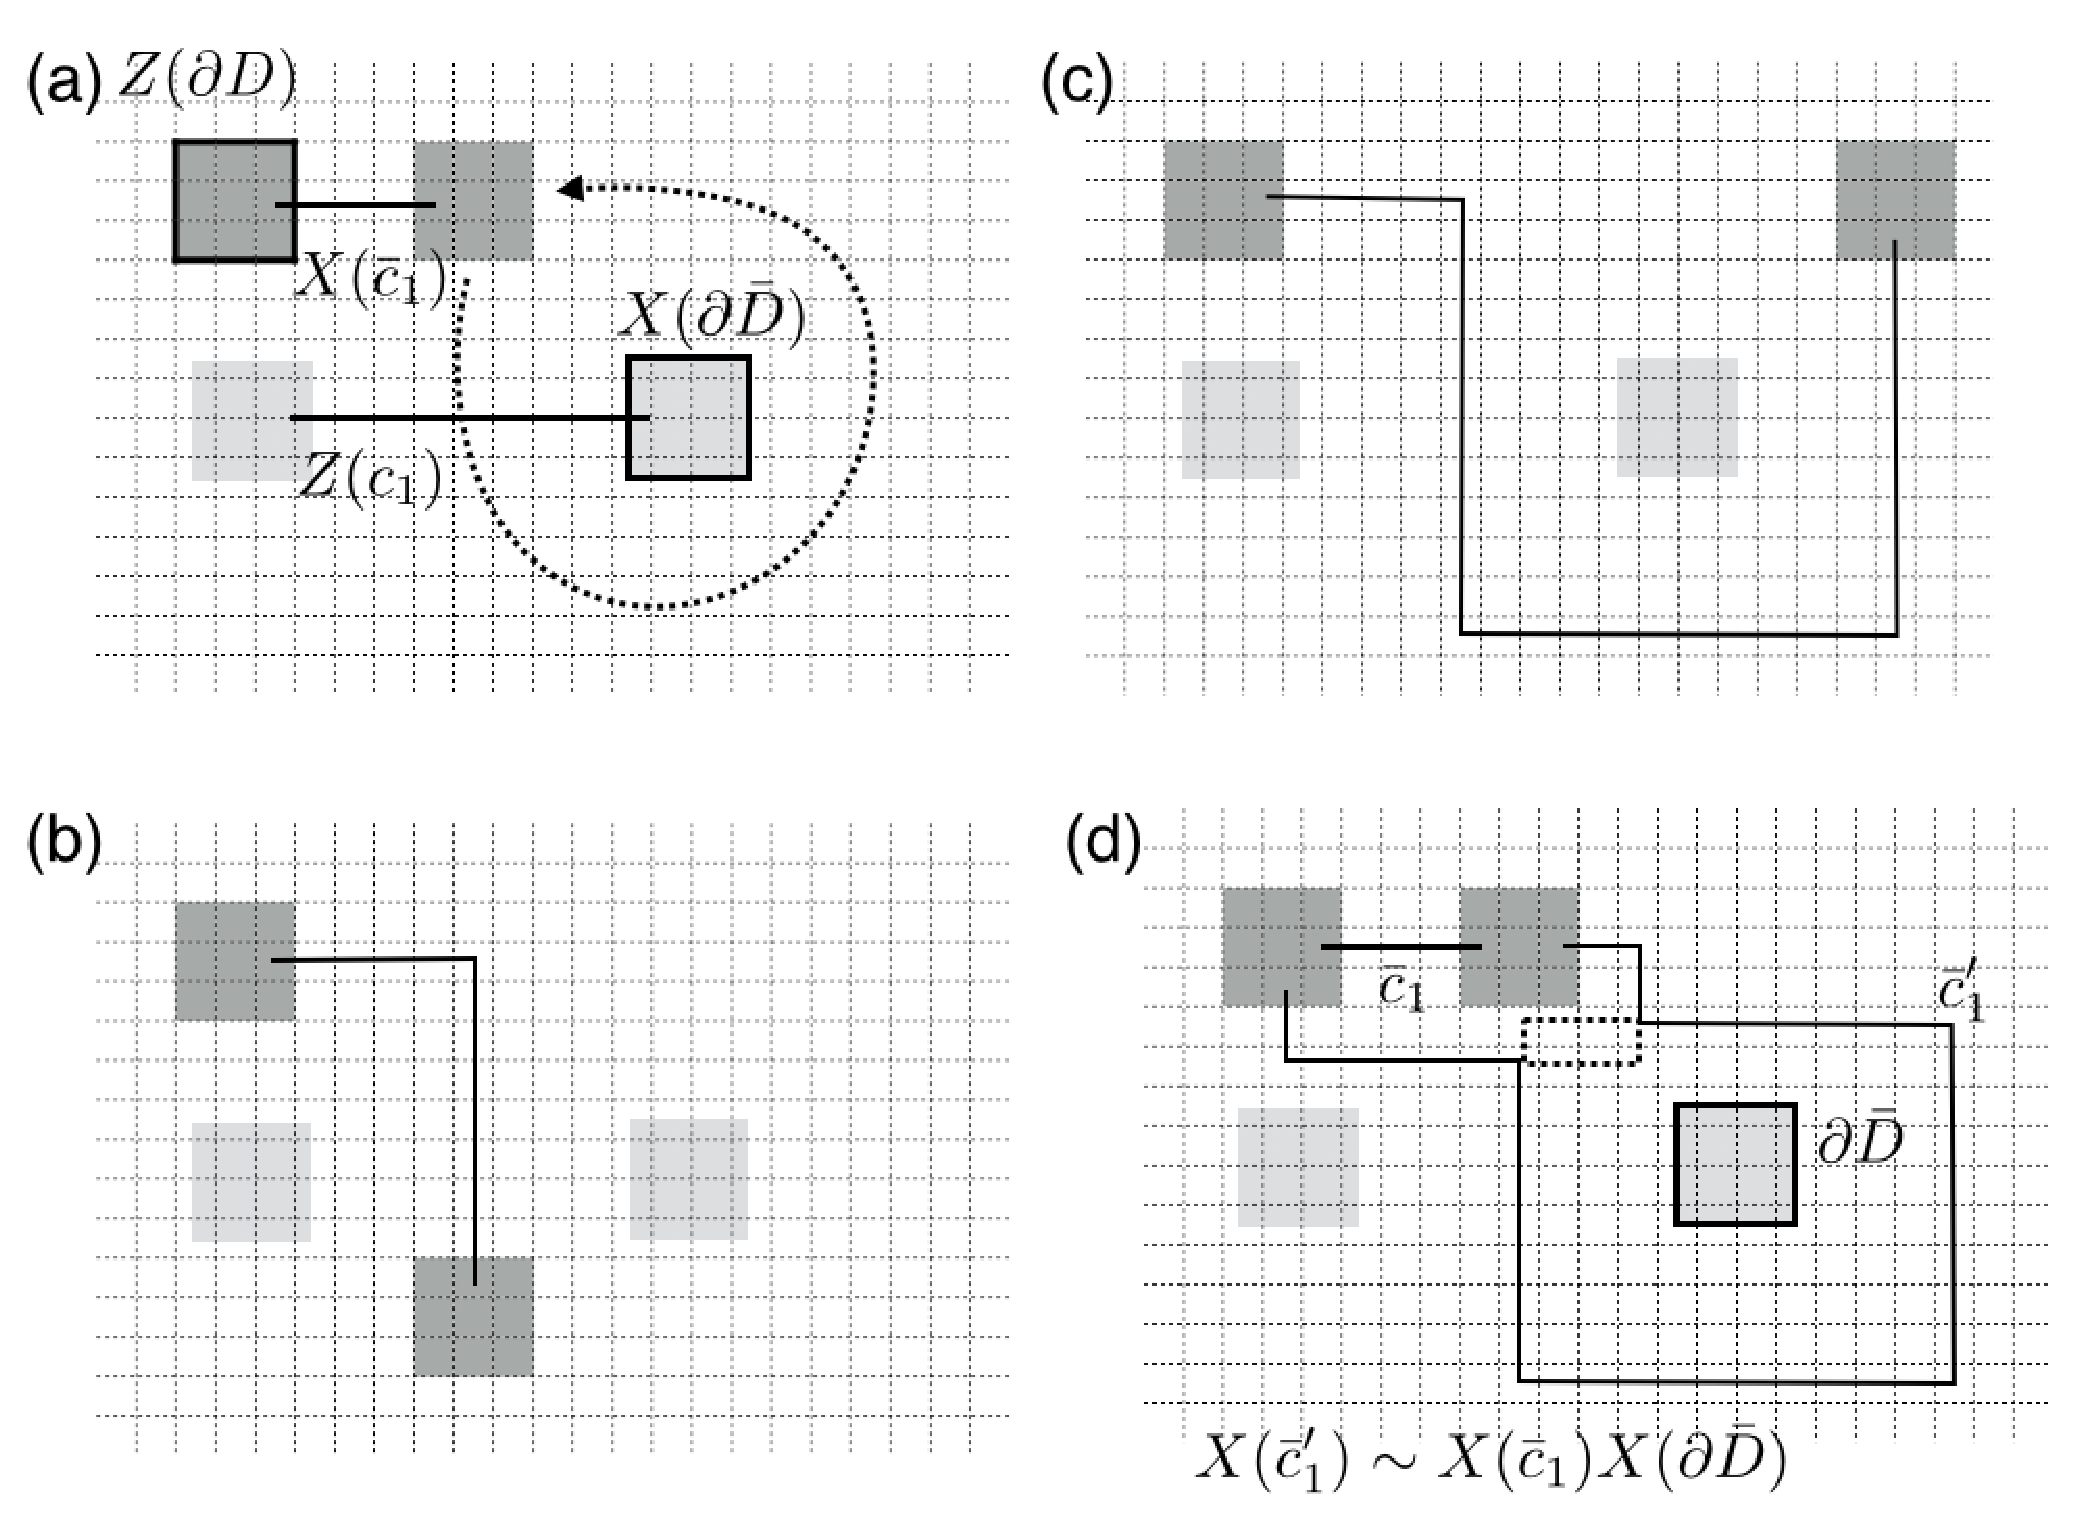
\includegraphics[width=150mm]{fig75.eps}
%
% If not, use
%\picplace{5cm}{2cm} % Give the correct figure height and width in cm
%
\caption{A logical CNOT gate created by braiding. 
(a) A primal defect is braided around a dual defect. 
(b,c) The logical $X$ operator is deformed continuously during the braiding operations. 
(d) After the braiding, the logical $X$ operator is represented by the dual chain $\bar c_1'$ winding around the primal defect.
By applying star operators inside the rectangle denoted by dotted lines, $\bar c_1'$ is decoupled into a chain connecting two primal defects and a chain surrounding the dual defect. 
The corresponding operators are equivalent to the products of the logical $X$ operators on the primal and dual qubits.
}
\label{fig75}       % Give a unique label
\end{figure}
We first consider the CNOT gate between primal (control) and dual (target) defect pair qubits.
Suppose there are primal and dual qubits on the surface code as shown in Fig.~\ref{fig75} (a), where logical operators are specified by the chains $\{ \partial D, \bar c_1\}$ 
and $\{ \partial \bar D,  c_1\}$ for the primal and dual qubits, respectively.
We can freely move the defect everywhere we want by the defect expansion and contraction.
Let us braid the primal defect around the dual defect, as shown in Fig.~\ref{fig75} (a)-(d).
After the braiding operation, the operator $X(\bar c_1')$ in Fig.~\ref{fig75} (d) 
has the same information as the operator $X(\bar c_1)$ before the braiding.
Using the equivalence relation,
\begin{eqnarray}
X(\bar c_1') \sim  X(\bar c_1) X(\partial D),
\end{eqnarray}
we understand that a correlation is made by the braiding operation between the logical $X$ operators $X(\bar c_1)$ and $X(\partial D)$ of the primal and dual defect pair qubits.
\begin{figure}[t]
\centering
%\sidecaption
% Use the relevant command for your figure-insertion program
% to insert the figure file.
% For example, with the option graphics use
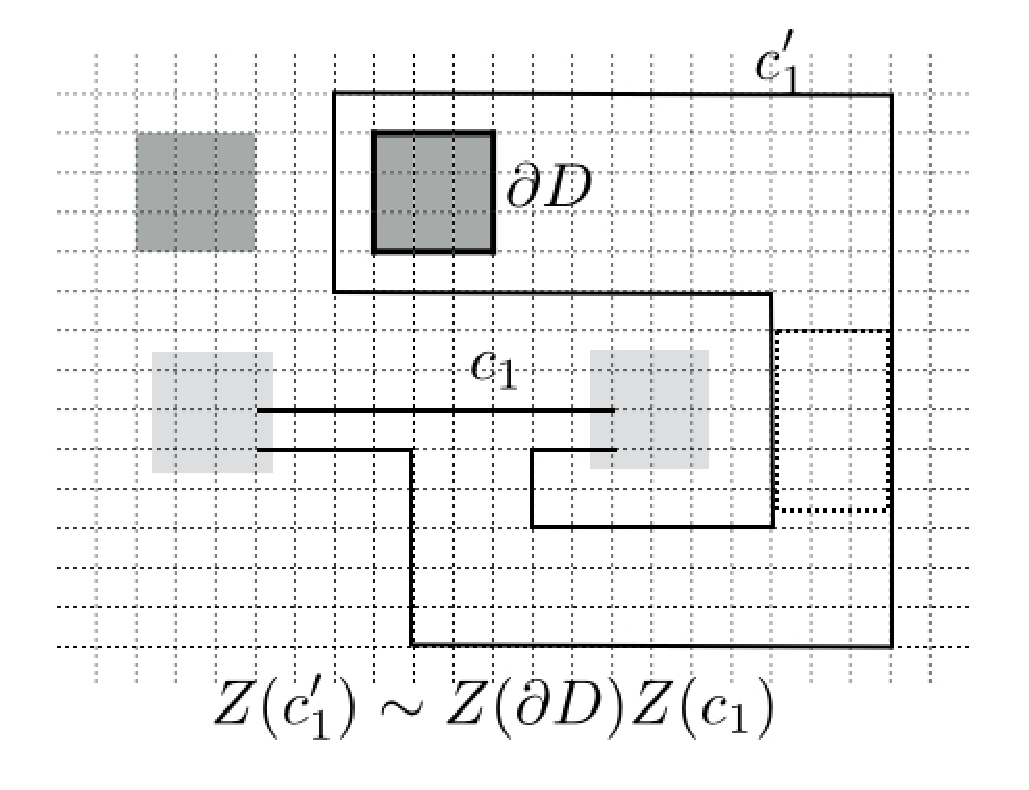
\includegraphics[width=90mm]{fig76.eps}
%
% If not, use
%\picplace{5cm}{2cm} % Give the correct figure height and width in cm
%
\caption{The time evolution of the logical $Z$ operator caused by braiding. 
The logical $Z$ operator on the dual qubit is transformed into the product of the logical $Z$ operators on the primal and dual qubits.}
\label{fig76}       % Give a unique label
\end{figure} 
A similar observation holds for the logical operator $Z(c_1)$, which is transformed into $Z(c_1') \sim Z(c_1) Z(\partial D)$ (see Fig.~\ref{fig76}).
On the other hand, $Z(\partial D)$ and $X(\partial \bar D)$ are invariant under this operation.
In short, the braiding operation transforms the logical Pauli operators as follows:
\begin{eqnarray}
Z(\partial D) &\rightarrow& Z(\partial D),
\label{eq:braid_CNOT1}
\\
Z(c_1) &\rightarrow& Z(c_1) Z(\partial D),
\label{eq:braid_CNOT2}
\\
X(\partial \bar D) &\rightarrow & X(\partial \bar D),
\label{eq:braid_CNOT3}
\\
X(\bar c_1) &\rightarrow& X(\bar c_1) X(\partial \bar D).
\label{eq:braid_CNOT4}
\end{eqnarray}
This transformation is equivalent to that for the CNOT gate, Eqs.\ (\ref{eq:CNOT1}-\ref{eq:CNOT4}).
Thus, braiding the primal defect around the dual defect results in a logical CNOT gate between the primal and dual defect pair qubits.

\begin{figure}[t]
\centering
%\sidecaption
% Use the relevant command for your figure-insertion program
% to insert the figure file.
% For example, with the option graphics use
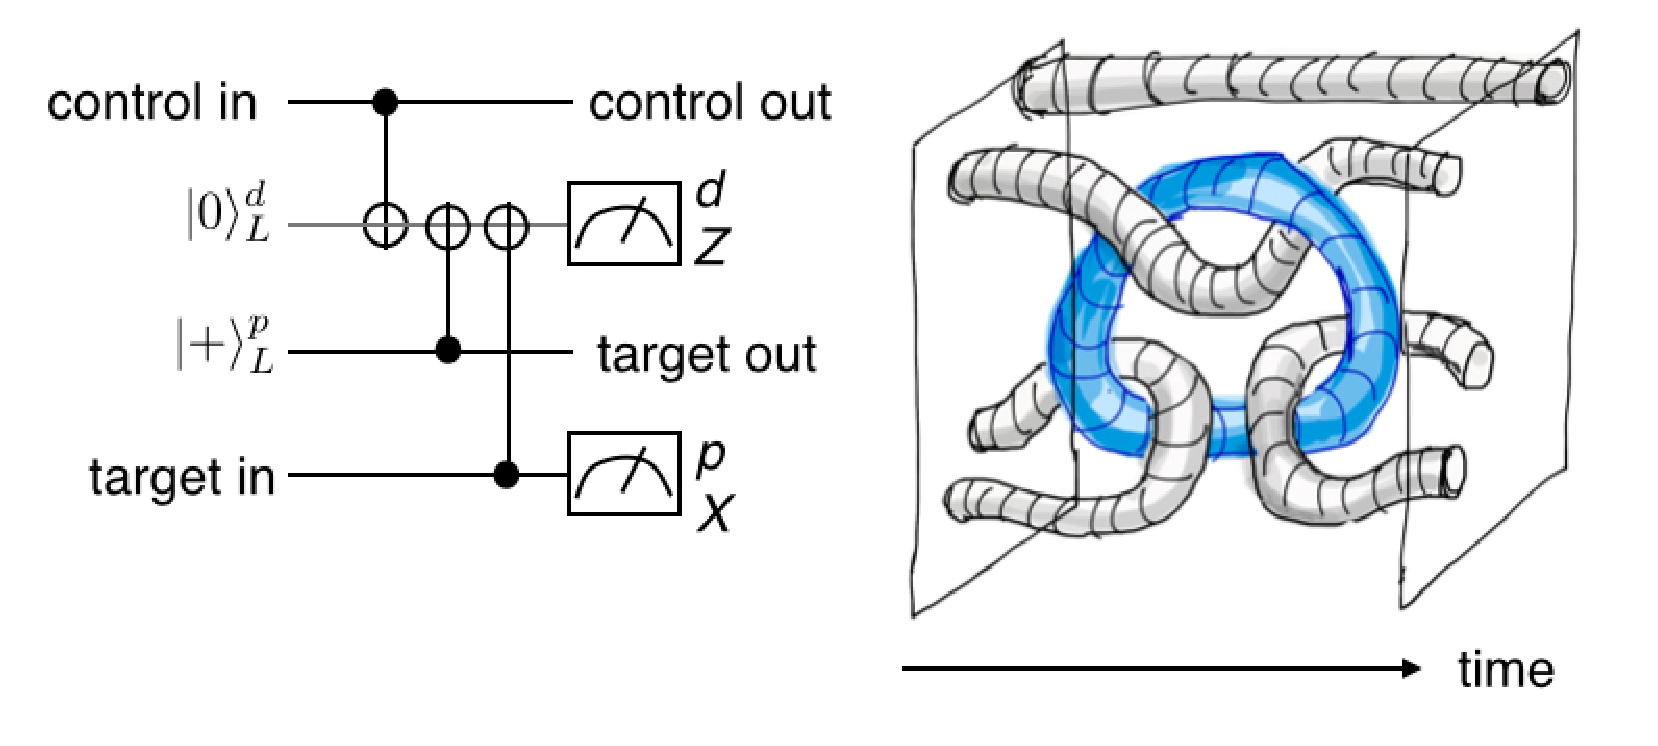
\includegraphics[width=140mm]{fig77.eps}
%
% If not, use
%\picplace{5cm}{2cm} % Give the correct figure height and width in cm
%
\caption{The circuit diagram of the teleportation-based CNOT gate between primal qubits using a dual qubit as ancilla (left). 
The control and target qubits of the CNOT gates are always primal and dual qubits, respectively. The corresponding braiding operation (right).
}
\label{fig77}       % Give a unique label
\end{figure}
Unfortunately, in the above CNOT gate, the primal (dual) defect is always a control (target) qubit.
Such CNOT gates always commute with each other, which is a natural consequence of the fact that the defect qubits on the surface code are Abelian.
In order to realize a genuine CNOT gate between the same type of qubits (and hence noncommuting gates), we utilize a teleportation-based gate \cite{GottesmanChuang}, as shown in Fig. \ref{fig77}.
Only CNOT gates between primal (control) and dual (target) qubits are employed.
The Pauli basis measurements are also done as mentioned in the previous section.
Accordingly, the CNOT gate between primal qubits is realized by braiding the primal defects around {\it virtual} dual defects, which are created and annihilated as ancillae.

The above braiding operations are implemented with topological quantum error correction at each elementary step, which will be explained later in detail.
All operations considered so far can be executed keeping the defect size (circumference) and defect distance larger than a length $d$, which provides a code distance of the logical qubits.
Thus, the logical error probability for the logical CNOT gates decreases exponentially by increasing the characteristic length $d$ of the system.
In other words, the CNOT gates are topologically protected.

We should mention that 
the braiding operations explained above are not the only way to 
perform fault-tolerant operations on the surface code.
There are another approaches to perform logical operations 
fault-tolerantly for the encoded degrees of freedom of the surface code.
One is the lattice surgery scheme~\cite{Horsman12},
where the boundary conditions of two planar surface codes 
are engineered to perform a logical operation.
Another is to employ twists,
which are topological defects introduced by
point defects on lattices~\cite{BombinTwist,Bombin11}.
All Clifford gates can be implemented by the
twist creation, braiding, and annihilation
similarly to the defect pair qubits explained above.
All these different approaches 
can be view as the logical operations by the code deformations~\cite{Dennis,RaussendorfAnn,Bombin09}
and seem to be a unique feature 
for the topological codes 
contrasting to the transversal logical gate for the concatenated codes.

\section{Magic state injections and distillation}
\label{Sec:MagicInjection}
Unfortunately, the topologically protected CNOT gates do not allow universal quantum computation, because Clifford circuits can efficiently be simulated classically due to the Gottesman-Knill theorem~\cite{GottesmanKnill}.
Here, we explain how to perform single-qubit rotations on the defect pair qubit, while, unfortunately, they are not topologically protected.

\begin{figure}[t]
\centering
%\sidecaption
% Use the relevant command for your figure-insertion program
% to insert the figure file.
% For example, with the option graphics use
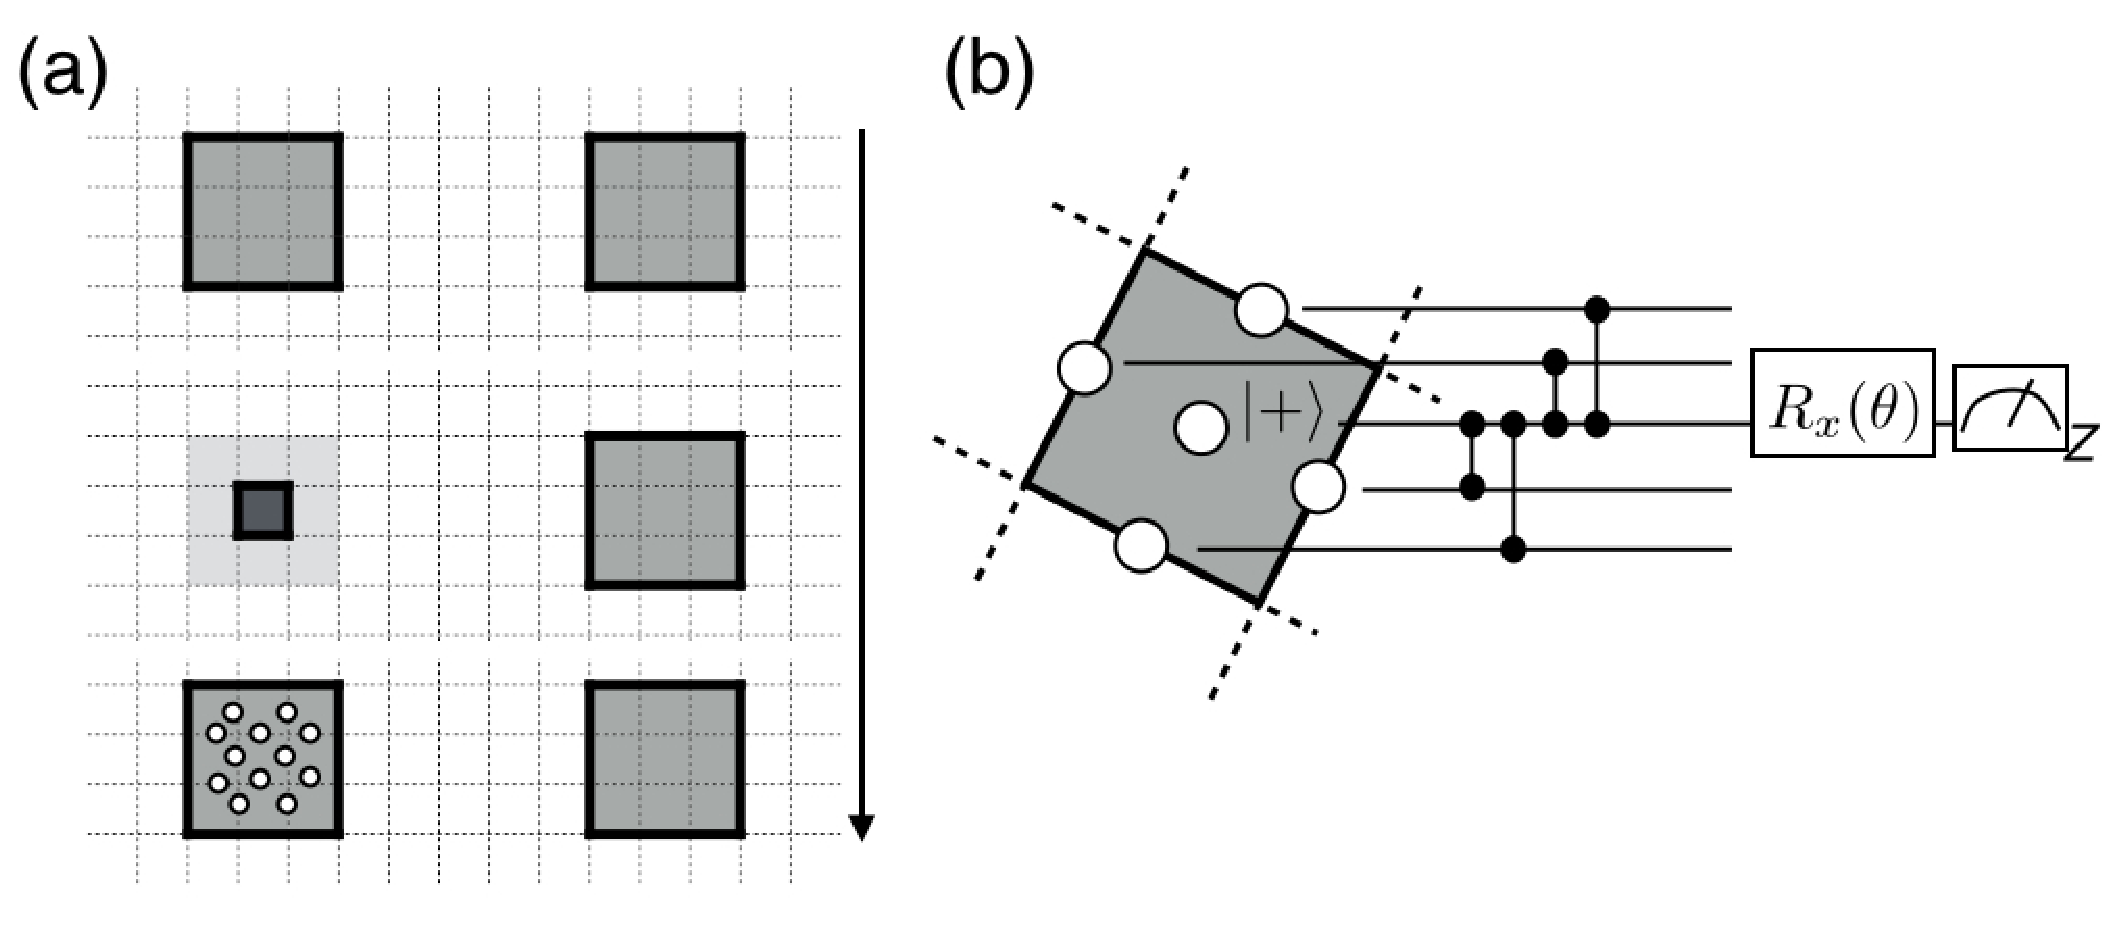
\includegraphics[width=130mm]{fig80.eps}
%
% If not, use
%\picplace{5cm}{2cm} % Give the correct figure height and width in cm
%
\caption{(a) A magic state injection by contracting the defect into 
an elementary cell. 
(b) A circuit diagram for the logical $Z$ rotation on the defect of an elementary cell.}
\label{fig80}       % Give a unique label
\end{figure}
Suppose we have a defect pair qubit, whose logical operators are given by $Z(\partial D)$ and $X(c_1)$.
We first consider a logical $Z$ rotation $e^{-i (\theta/2) Z(\partial D)}$ on the defect pair qubit.
To this end, the defect region $D$ is contracted to a single face $f_l$ by using the annihilation process, as shown in Fig.~\ref{fig80} (a).
Now the logical operator $Z(f_l)$ is a four-body operator.
(This implies that the code distance becomes 4 at this stage.)
A rotation with respect to the logical operator $Z(f_l)$, $e^{-i (\theta/2) Z(f_l)}$, can be implemented 
indirectly by using an acilla qubit located at the center of the face
shown in Fig.~\ref{fig80} (b).
First, the four CZ gates are applied 
between the ancilla and the four edge qubits on the face.
Second, after applying a $X$-rotation $R_x(\theta )= e^{-i (\theta/2) X}$,
the ancilla qubit is measured in the $Z$-basis. 
According to the measurement outcome $m=0,1$,
a logical rotation $e^{-i(-1)^{m} (\theta/2) Z(f_l)}$ is implemented.
After the above procedure, the defect, as a single face $f_l$, is expanded again into the defect region $D$ to restore the code distance of the defect pair qubit.

\begin{figure}[t]
\centering
%\sidecaption
% Use the relevant command for your figure-insertion program
% to insert the figure file.
% For example, with the option graphics use
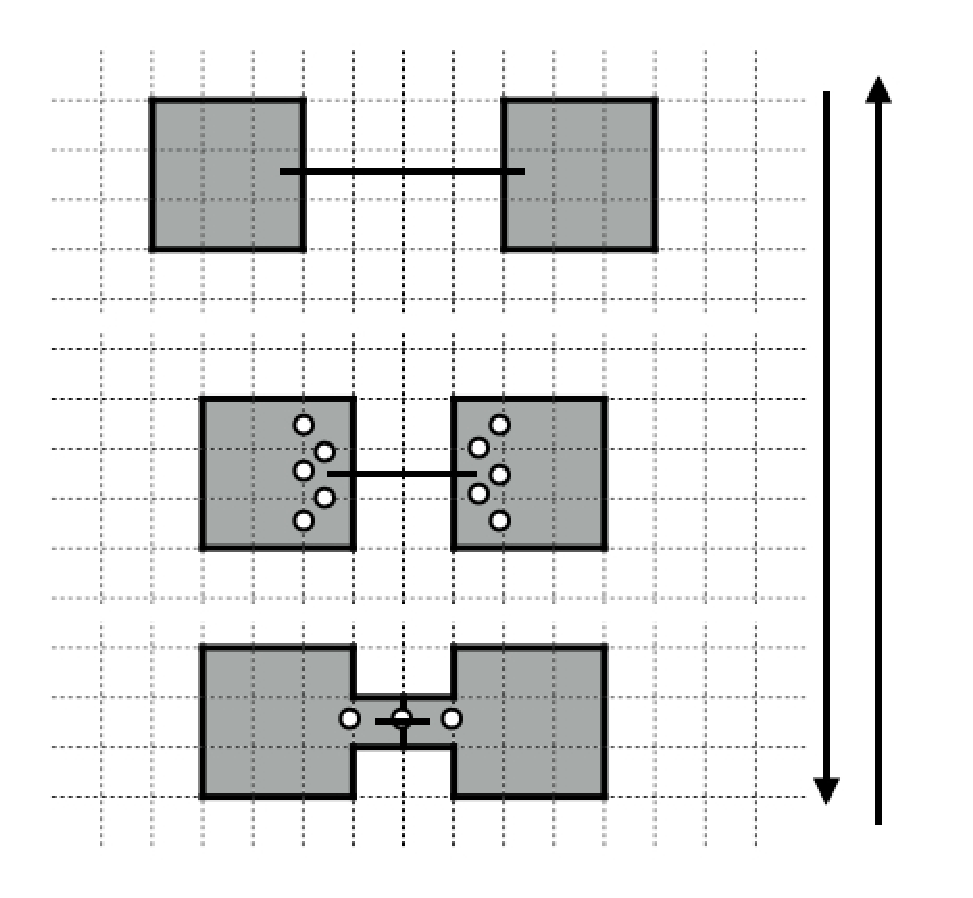
\includegraphics[width=90mm]{fig81.eps}
%
% If not, use
%\picplace{5cm}{2cm} % Give the correct figure height and width in cm
%
\caption{A magic state injection by connecting two defects.
If two defects regions are adjacent, the logical $X$ operator is a physical Pauli $X$ operator between two defects.}
\label{fig81}       % Give a unique label
\end{figure}
Next we consider a logical $X$ rotation, $e^{-i (\theta/2) X(c_1)}$.
In this case, the two defects are moved and deformed near each other such that $X(c_1')$ becomes a one-body operator as shown in Fig.~\ref{fig81}.
The rotation $e^{-i (\theta/2) X(c_1')}$ is now easily implemented by a single-qubit gate.
After that, the distance between two defects is restored.

\begin{figure}[t]
\centering
%\sidecaption
% Use the relevant command for your figure-insertion program
% to insert the figure file.
% For example, with the option graphics use
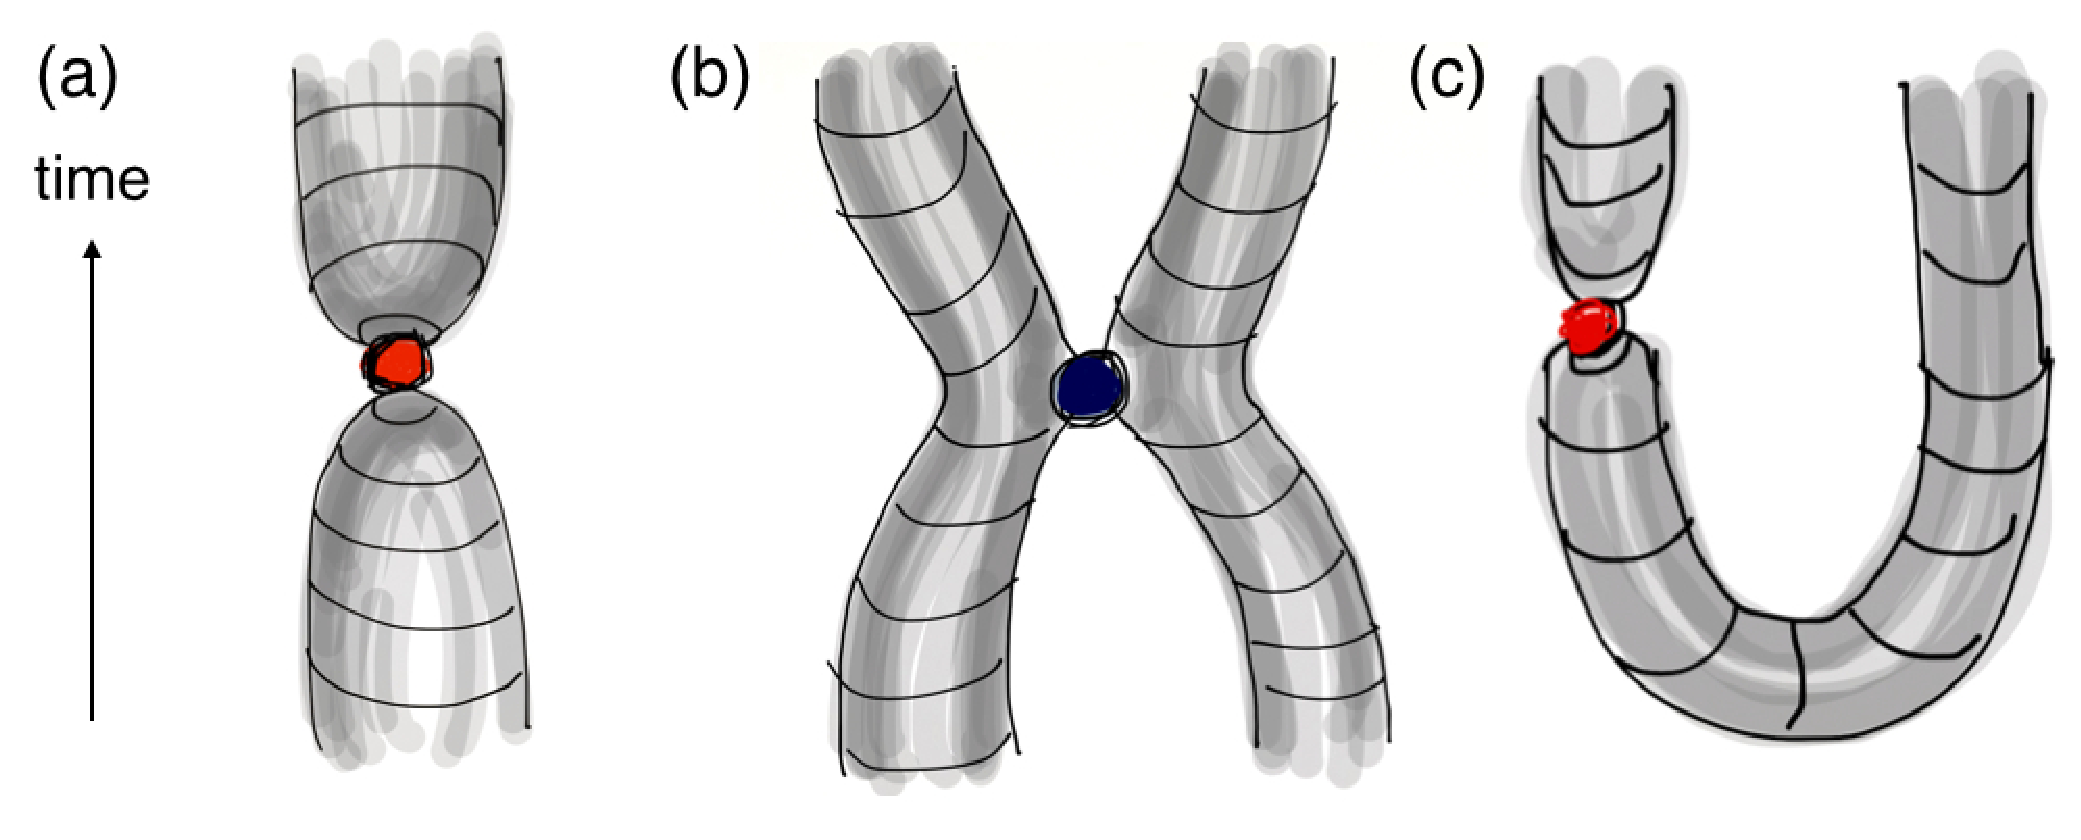
\includegraphics[width=110mm]{fig125.eps}
%
% If not, use
%\picplace{5cm}{2cm} % Give the correct figure height and width in cm
%
\caption{(a) The logical $Z$ rotation. (b) The logical $X$ rotation. (c) The logical 
$e^{-i (\theta /2)Z}|+\rangle$ state injection.}
\label{fig125}       % Give a unique label
\end{figure}
In this way, we can perform an arbitrary single-qubit unitary operation on the defect pair qubit by continuously deforming the defect pair qubit.
These deformations and the operations for the logical rotations
are depicted in Fig.~\ref{fig125}.
Unfortunately, during the deformation, the code distance inevitably becomes relatively small, so that we can perform logical rotations directly with nearest-neighbor operations.
Thus, these processes are not topologically protected.

These non-topological operations can be utilized to inject noisy magic states on the surface.
Specifically, the logical $e^{-i(\theta/2)Z}|+\rangle$ state
is injected as shown in Fig.~\ref{fig125} (c).
Then, these noisy magic states are distilled by topologically protected operations 
to clean magic states, which have a fidelity high enough for reliable quantum computation.
Note that we are allowed to use only the CNOT gates, and there is no topologically protected single-qubit Clifford gate.
To manage this, we distill two types of magic states.
One is the eigenstate of the Pauli-$Y$ operator, which is used to implement the $S$ gate via gate teleportation~\cite{GottesmanChuang,Leung}, as shown in Fig.~\ref{fig82} (a).
Another is the eigenstate of the $(X+Y)/\sqrt{2}$ operator, which is used to implement the $\pi/8$ gate, a non-Clifford gate necessary for universal quantum computation.
The magic state distillation for the $Y$-basis state is executed solely by the topologically protected CNOT gates using the Steane 7-qubit code,
similarly to the method introduced in Sec.~\ref{sec:magic}.
The topologically protected CNOT gates and the $S$ gates with the distilled $Y$-basis states are further employed to distill the $(X+Y)/\sqrt{2}$-states through the Reed-Muller 15-qubit code, as explained in Sec.~\ref{sec:magic}.
\begin{figure}[t]
\centering
%\sidecaption
% Use the relevant command for your figure-insertion program
% to insert the figure file.
% For example, with the option graphics use
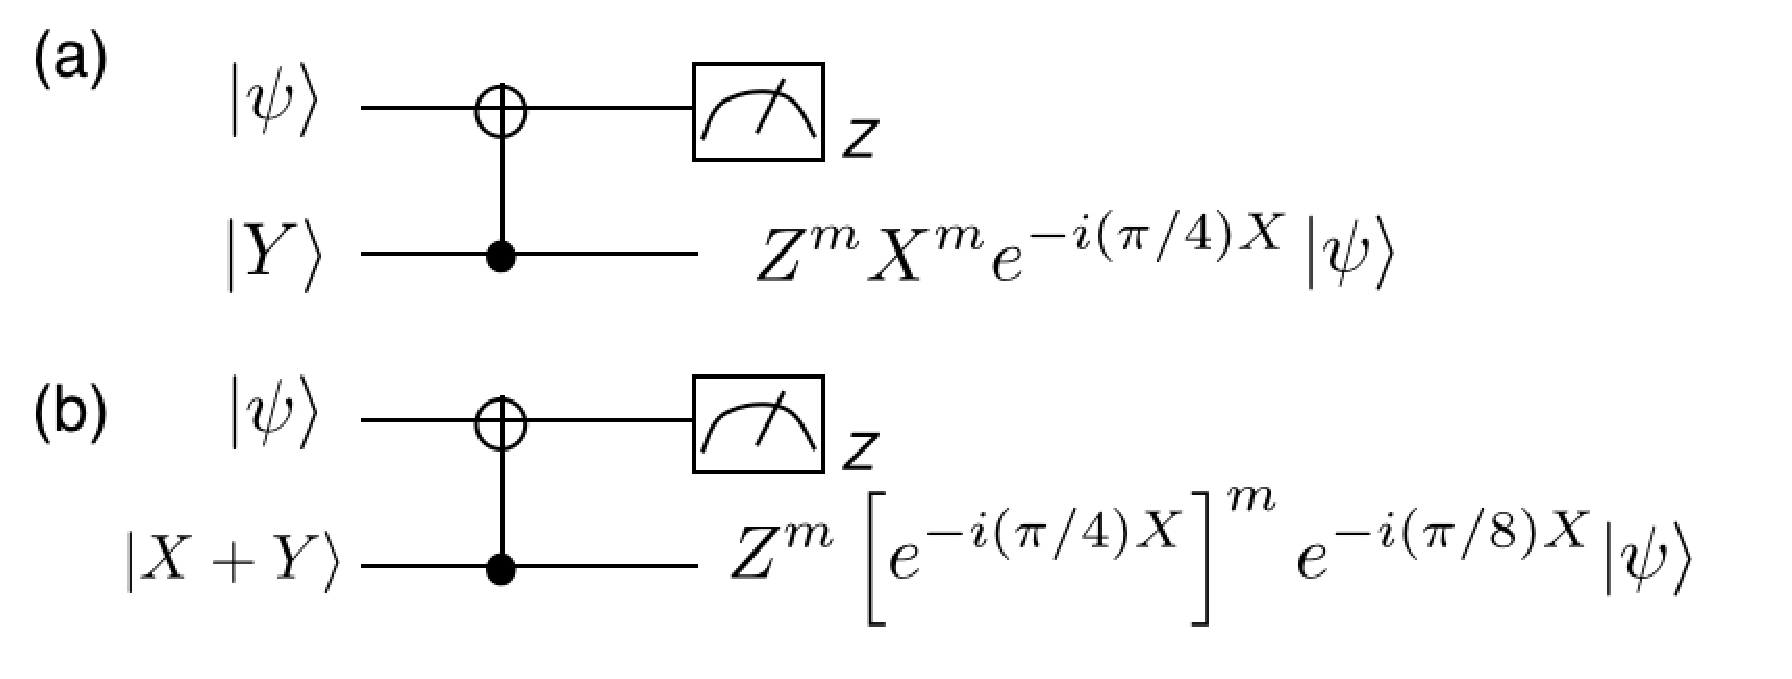
\includegraphics[width=110mm]{fig82.eps}
%
% If not, use
%\picplace{5cm}{2cm} % Give the correct figure height and width in cm
%
\caption{(a,b) Single-qubit rotations by one-bit teleportations~\cite{Leung}.}
\label{fig82}       % Give a unique label
\end{figure}

Using these distilled magic states and the CNOT gates, we can implement the single-qubit gates shown in Fig.~\ref{fig82} (a) and (b), which together with the CNOT gate constitute a universal set of gates.
Accordingly, universal quantum computation is performed reliably on the surface code.
Note that all operations employed are single-qubit gates, two-qubit nearest-neighbor gates, and single-qubit measurements on the 2D array of qubits.

\section{Topological calculus}
\label{Sec:TopoCalc}
Based on the microscopic understanding of the topological operations, we can introduce a {\it topological diagram}\index{topological diagram} and a {\it topological calculus}\index{topological calculus}, 
which allows us a diagrammatic description 
of topological quantum computation on the surface codes.

In this diagram, the 3D space-time trajectory of the defects 
is depicted by projecting it onto a 2D plane
like link diagrams mentioned in Sec.~\ref{sec:JonesPoly}.
The trajectory of the primal and dual defects
as tubes in 3D space-time are denoted 
by pairs of solid and gray-colored lines:
\begin{center}
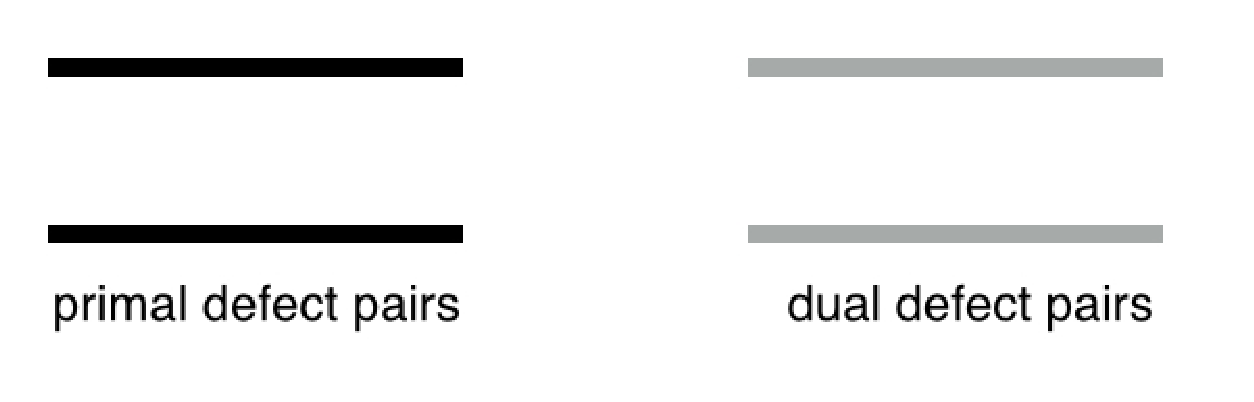
\includegraphics[width=90mm]{fig100.eps}
\end{center}
The braiding operation is denoted by a double crossing as follows:
\begin{center}
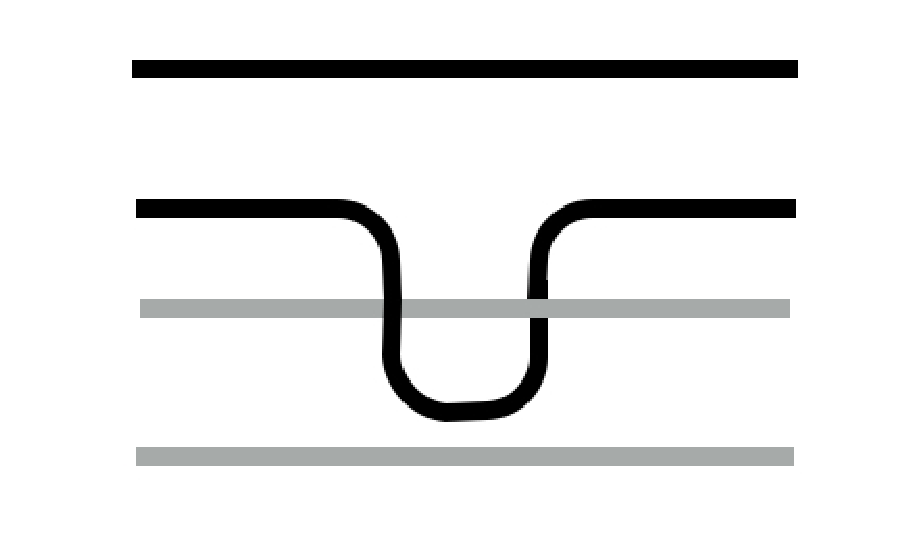
\includegraphics[width=70mm]{fig119.eps}
\end{center}
The logical $X$ state preparation and $X$-basis measurement of the primal defect are denoted by closures:
\begin{center}
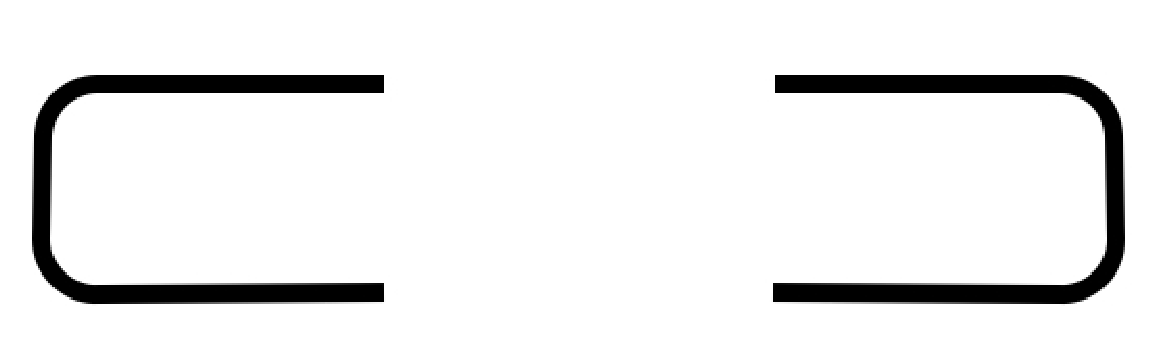
\includegraphics[width=70mm]{fig101.eps}
\end{center}
The logical $Z$ state preparation and $Z$-basis measurement of the primal defect are denoted by endpoints of the tubes:
\begin{center}
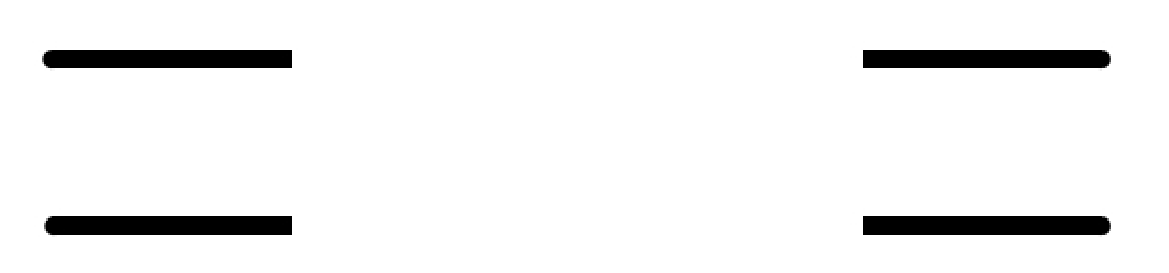
\includegraphics[width=70mm]{fig102.eps}
\end{center}
The state preparations and measurements for the dual defect pair qubit are depicted in a similar way with gray (curved) lines, except for the basis change by the Hadamard transformation.

The trajectories of the logical operators are represented by surfaces
in 3D space-time like a Seifert surface, 
which we call {\it correlation surfaces}\index{correlation surface}.
Specifically, the logical $Z$ operator for the primal defect corresponds to a surface wrapping around the primal defect.
The logical $X$ operator for the primal defect corresponds to a surface whose boundary is the primal defect tubes.
(This is also the case for the dual defect, except for the Hadamard transformation.)
For example, the time evolution of the logical $X$ and $Z$ operators by the braiding operation can be represented by the following surfaces
\begin{center}
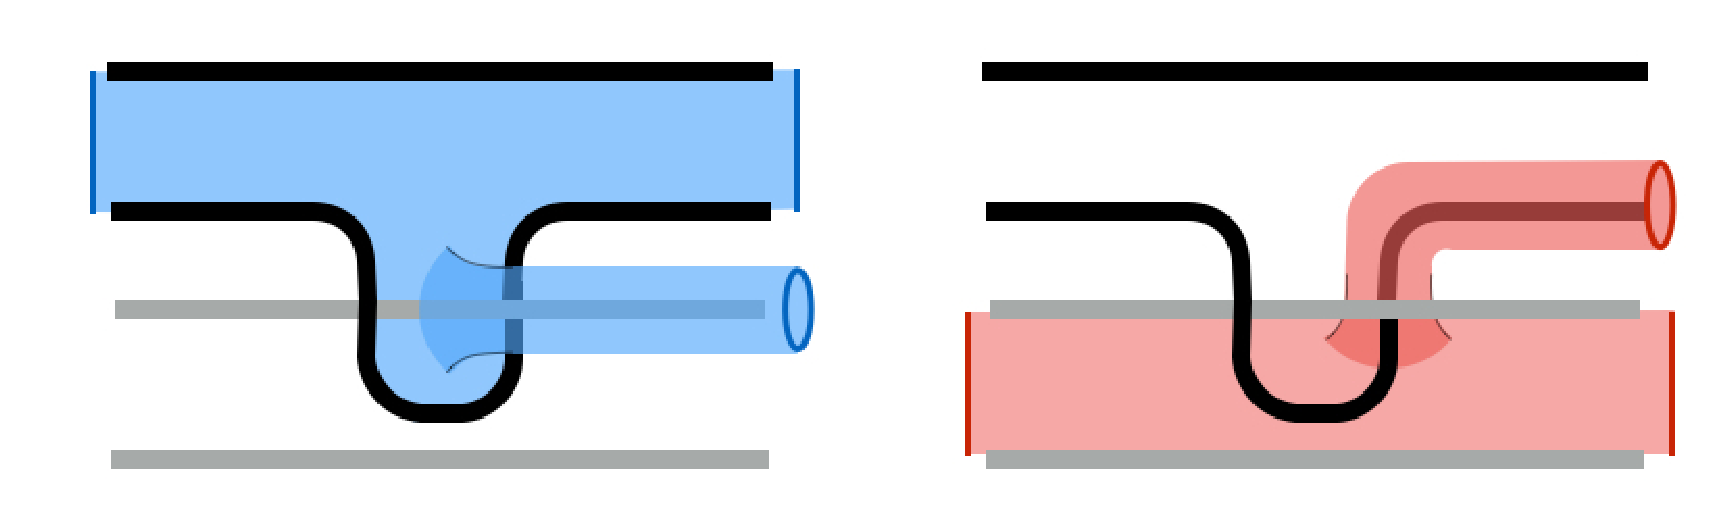
\includegraphics[width=100mm]{fig120.eps}
\end{center}
The logical operators before and after the operation correspond to the left and right boundaries of these surfaces, respectively.
We can confirm Eqs.~(\ref{eq:braid_CNOT1})-(\ref{eq:braid_CNOT4})
from the left and right boundaries the correlation surfaces of the above diagrams.

The CNOT gate between the primal defect pair qubits is depicted as follows:
\begin{center}
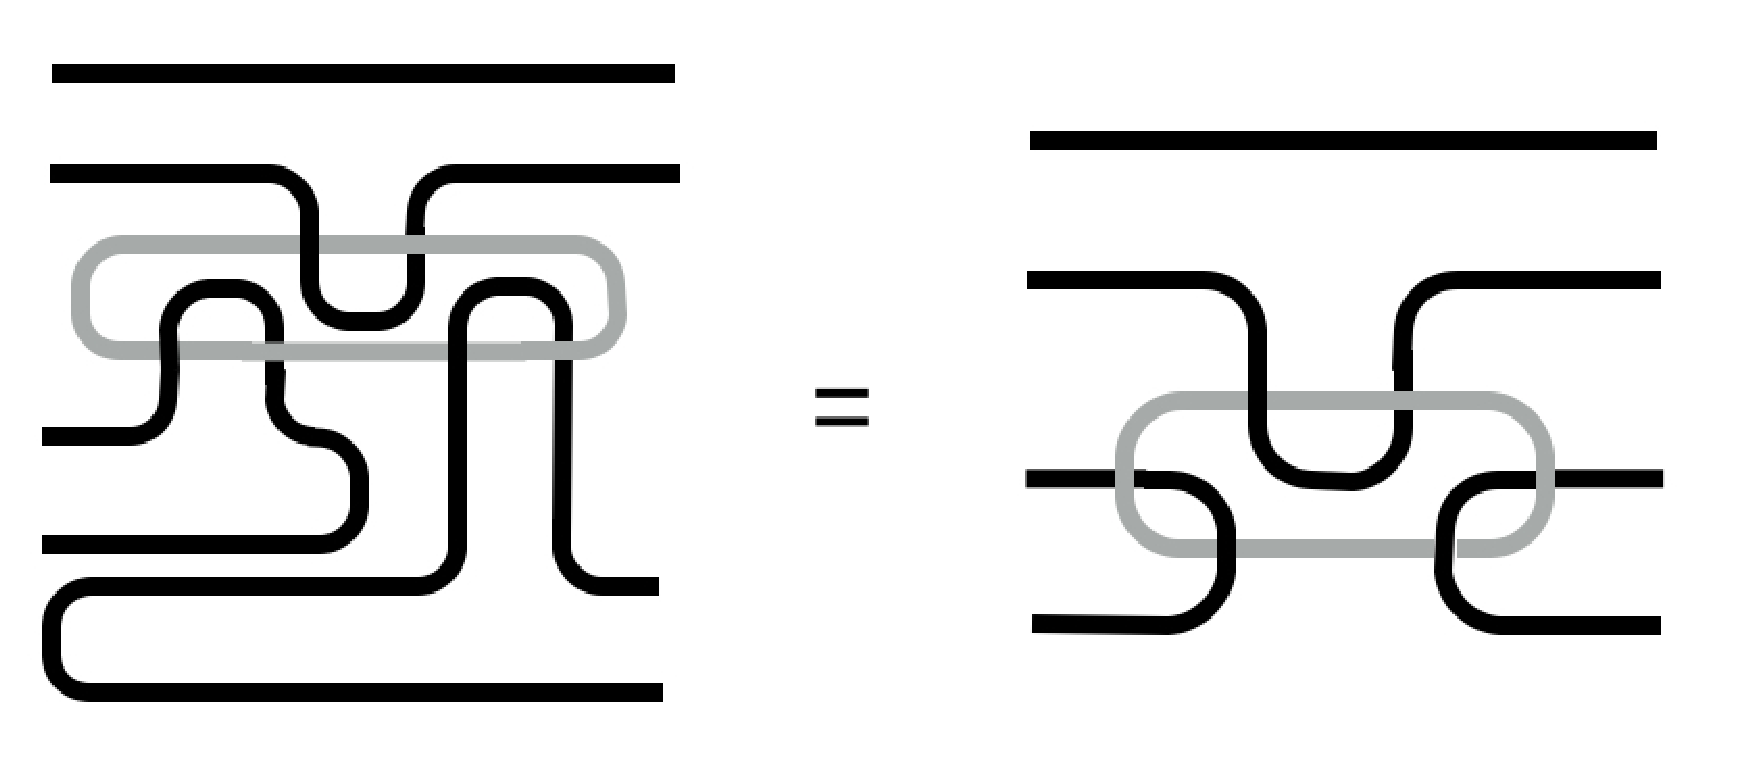
\includegraphics[width=120mm]{fig103.eps}
\end{center}
In this diagram, we can easily confirm that the braiding operations transform the logical operators according to the rule for the CNOT gate, i.e., 
$X\otimes I \rightarrow X\otimes X$ and $I \otimes Z \rightarrow Z \otimes Z$:
\begin{center}
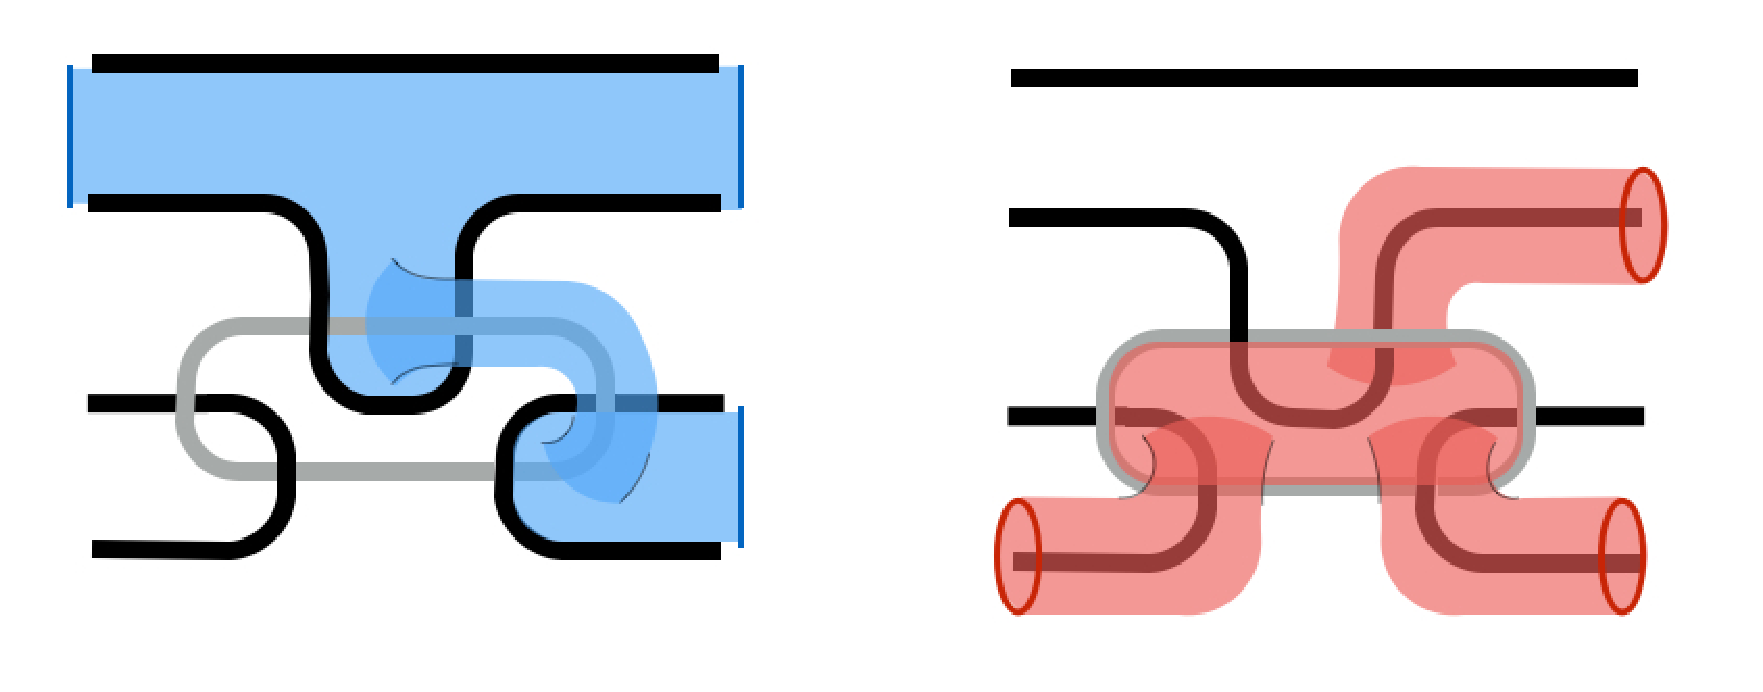
\includegraphics[width=120mm]{fig104.eps}
\end{center}

As seen above, the action on the code space is defined by the left and right boundaries of the correlation surfaces.
Thus, the logical action of the topological operation is invariant under transformations that do not change the topology of the left and right boundaries of the correlation surfaces. 
Similarly to link diagrams, the boundary topology is invariant under the Reidemeister moves\index{Reidemeister move}:
\begin{center}
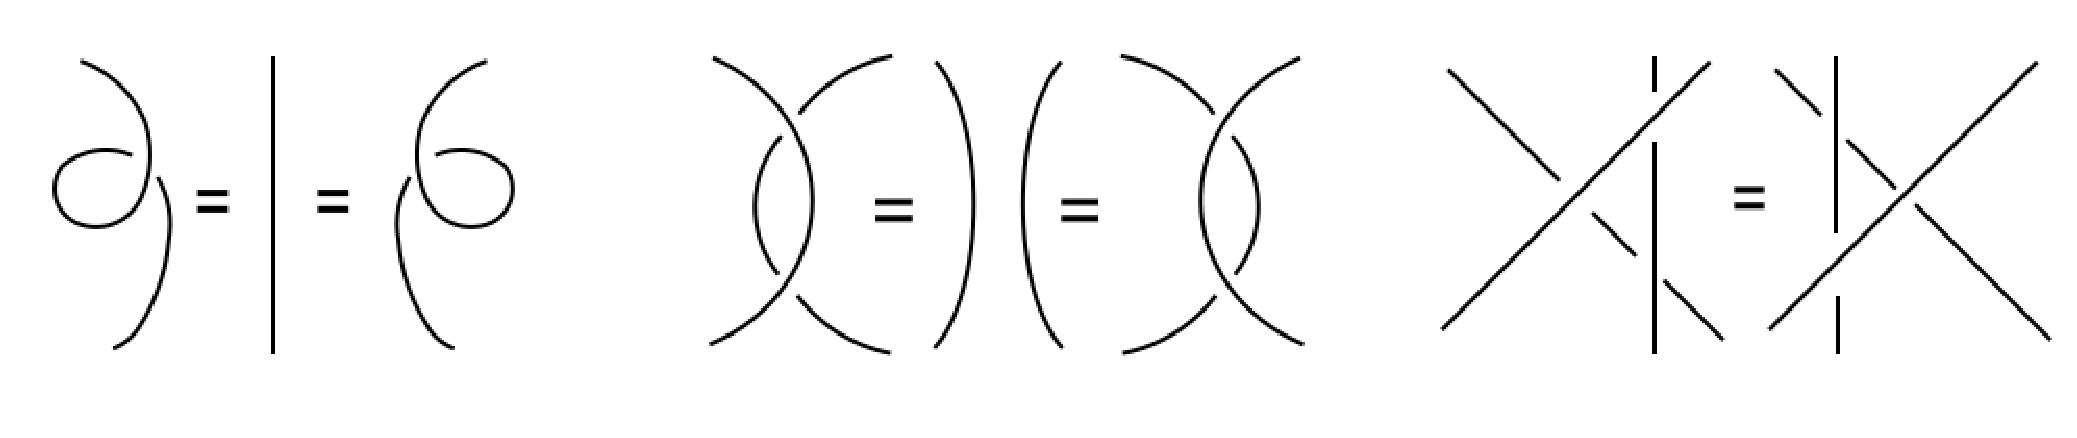
\includegraphics[width=140mm]{fig105.eps}
\end{center}
In the present case, we have further transformations under which the logical action on the code space is invariant due to the properties of the defect pair qubits.
At first, the following two crossings of tubes of the same type are equivalent:
\begin{eqnarray}
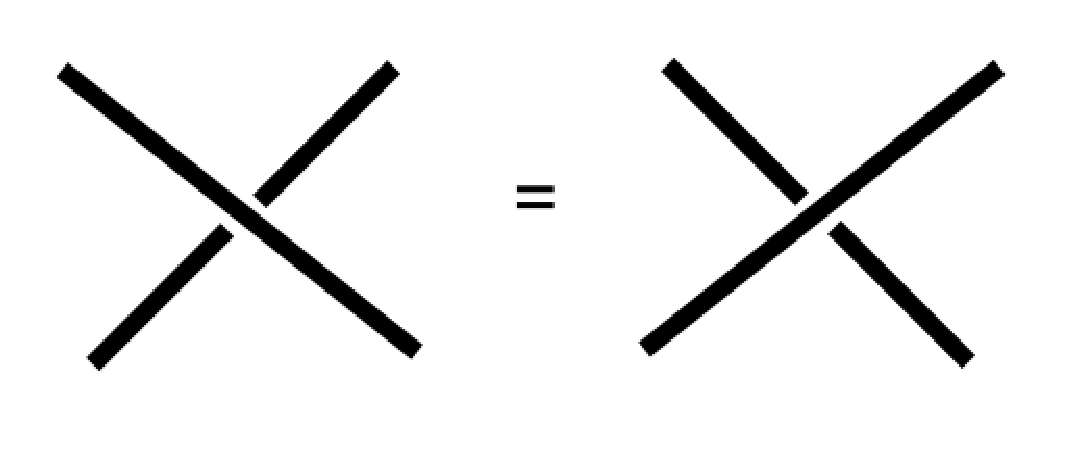
\includegraphics[width=80mm]{fig107.eps}
\label{TopoRule1}
\end{eqnarray}
Second, if two defect tubes are 
a defect pair qubit, a dual loop wrapping around a defect pair can be removed:
\begin{eqnarray}
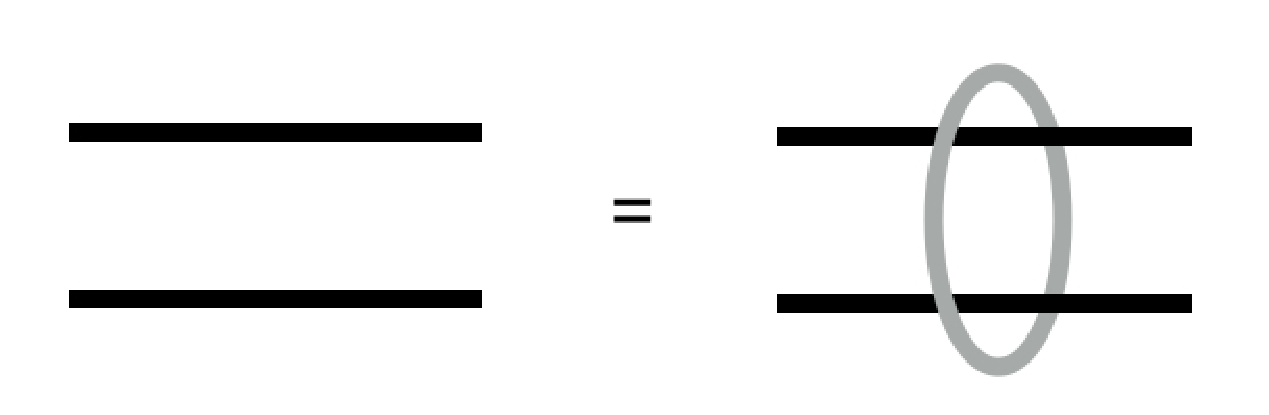
\includegraphics[width=80mm]{fig106.eps}
\label{TopoRule2}
\end{eqnarray}
This is because the primal defect pair qubit is stabilized by a $Z$-type loop operator surrounding the defect pair, and hence the dual loop is nothing but a trivial measurement of the stabilizer operator.
Third, because the defect pair qubit is a $\mathbf{Z}_2$ Abelian anyon, if we braid a primal defect around a dual defect twice, it results in an identity operation:
\begin{eqnarray}
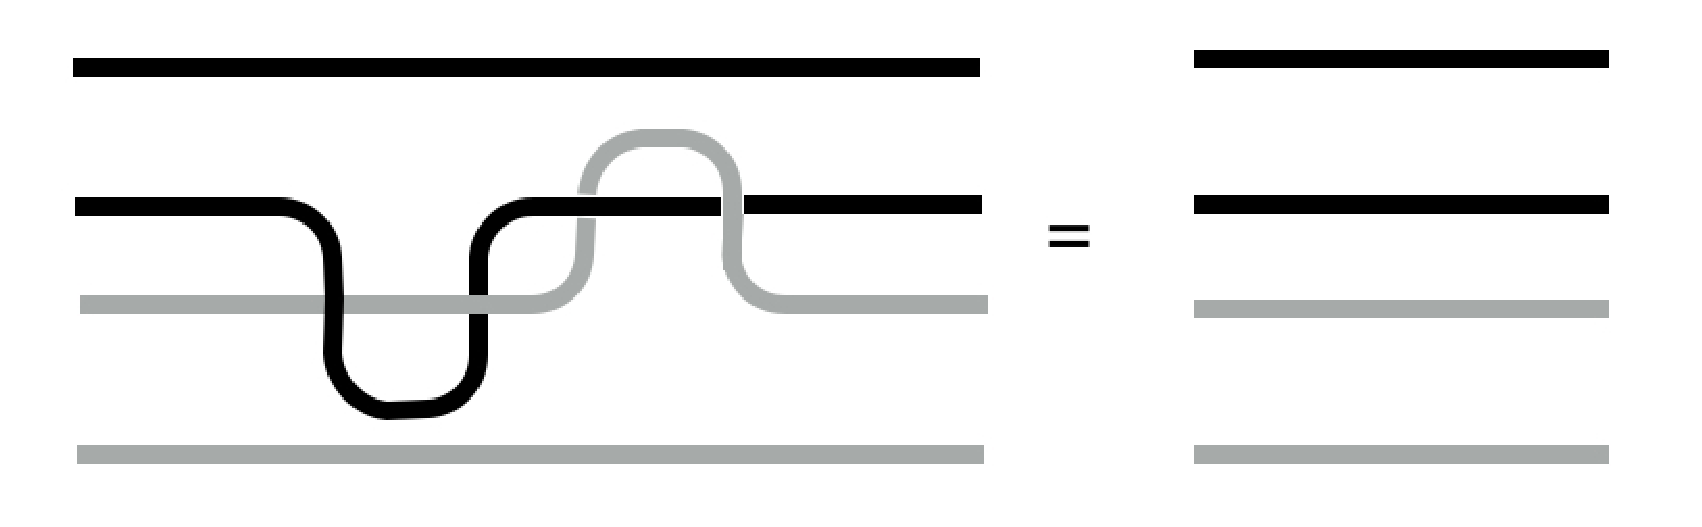
\includegraphics[width=100mm]{fig108.eps}
\label{TopoRule3}
\end{eqnarray}
Fourth, and most importantly, two tubes can be connected or disconnected by the following procedure, which we call a $\Phi$-transformation\index{$\Phi$-transformation}:
\begin{eqnarray}
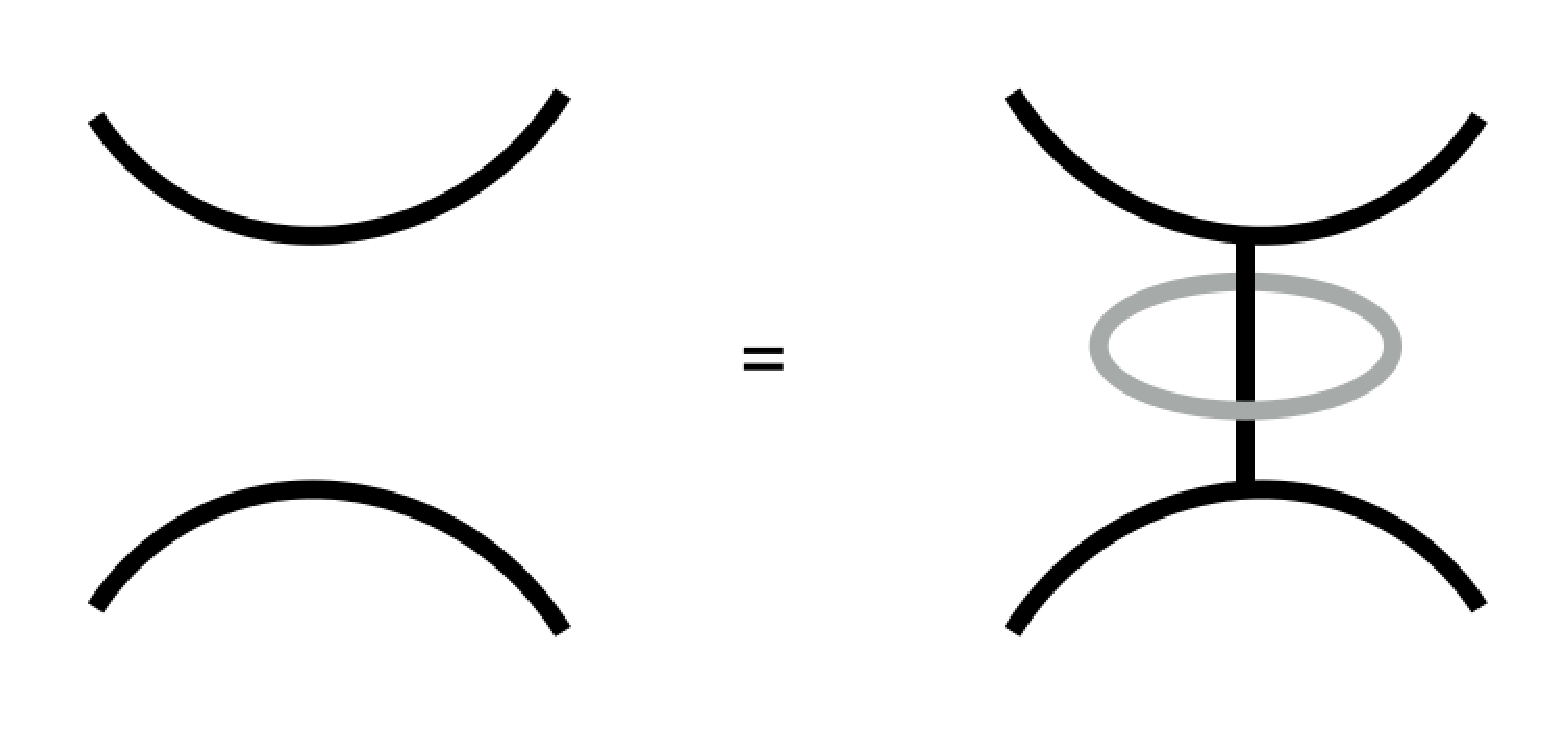
\includegraphics[width=90mm]{fig109.eps}
\label{TopoRule4}
\end{eqnarray}
We can easily confirm that the logical operators are invariant under the $\Phi$-transformation:
\begin{center}
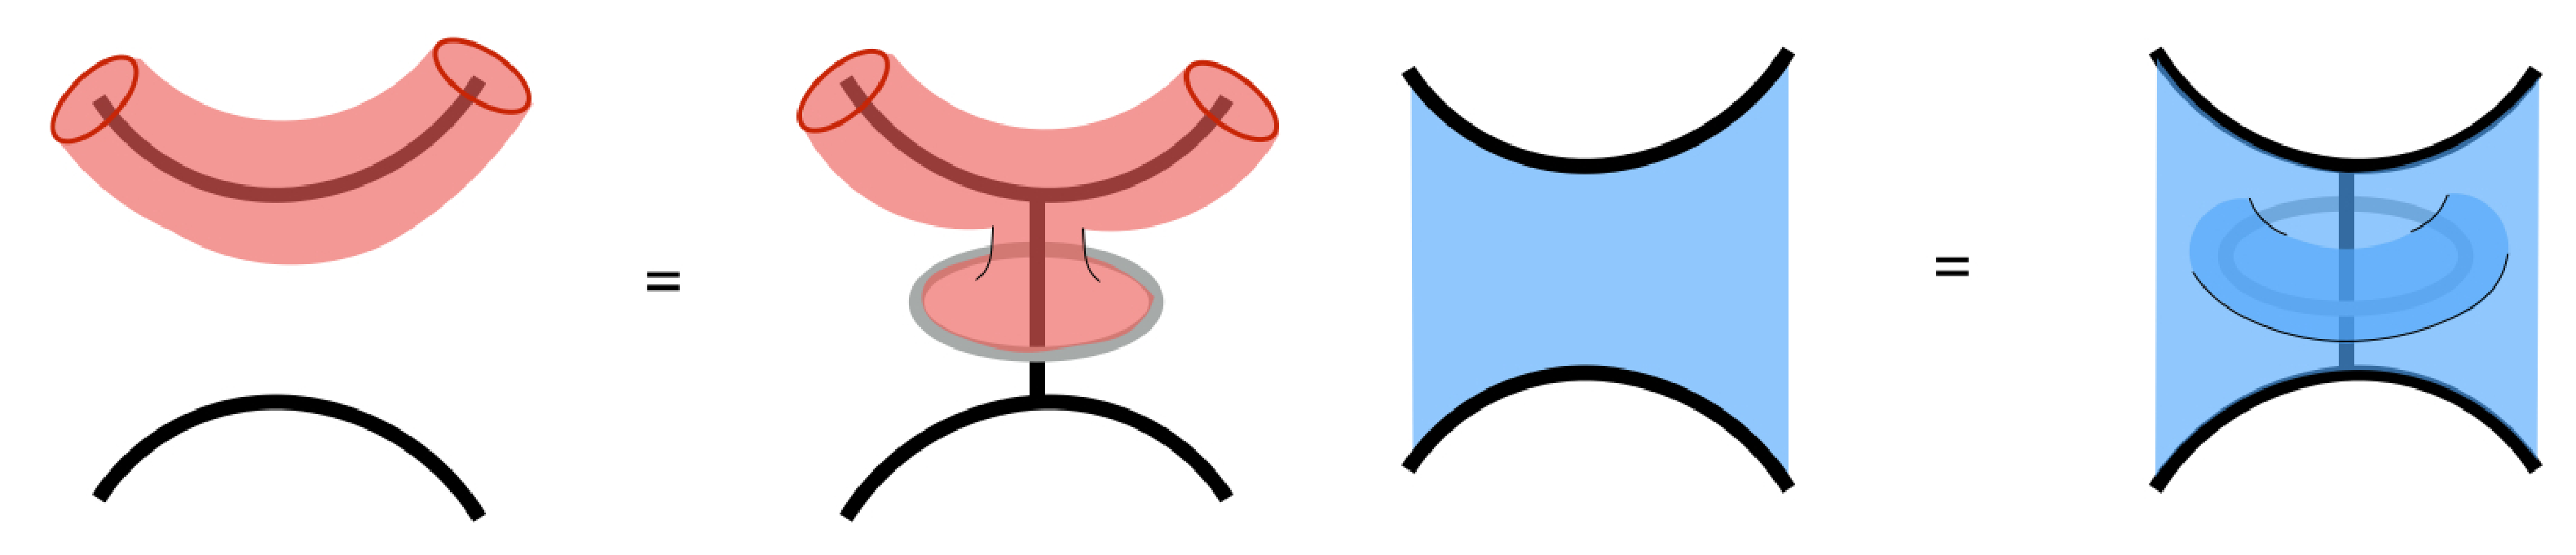
\includegraphics[width=120mm]{fig110.eps}
\end{center}
where we note that the dual ring in the middle serves to stop the $Z$-type correlation surface from propagating toward the bottom and also serves to mediate the $X$-type correlation surface toward the right.
Specifically, if two defect pair qubits are connected by the $\Phi$-transformation between their closures, we can remove the dual ring by using the rule (\ref{TopoRule3}):
\begin{center}
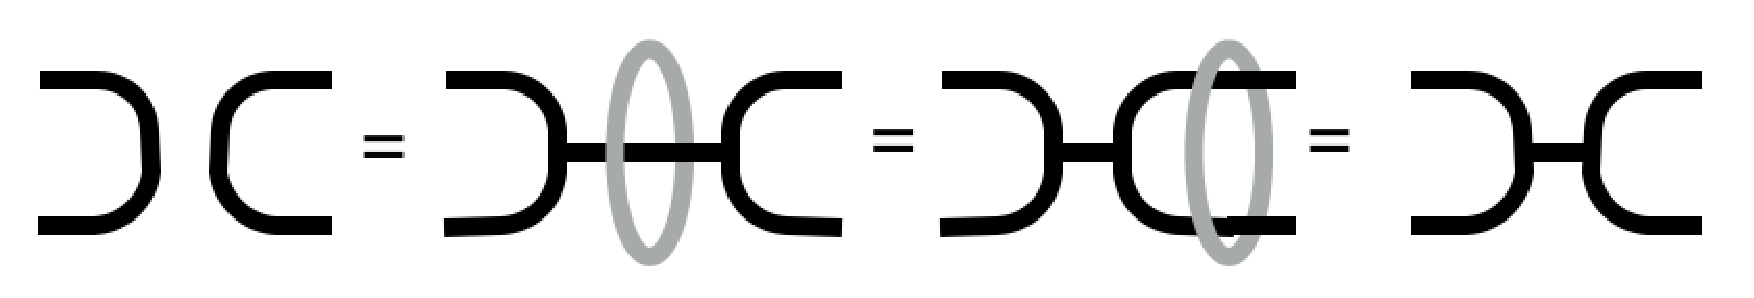
\includegraphics[width=120mm]{fig111.eps}
\end{center}
By using the $\Phi$-transformation and rules (\ref{TopoRule3}) and (\ref{TopoRule2}), we can transform the defect pair qubit as follows:
\begin{center}
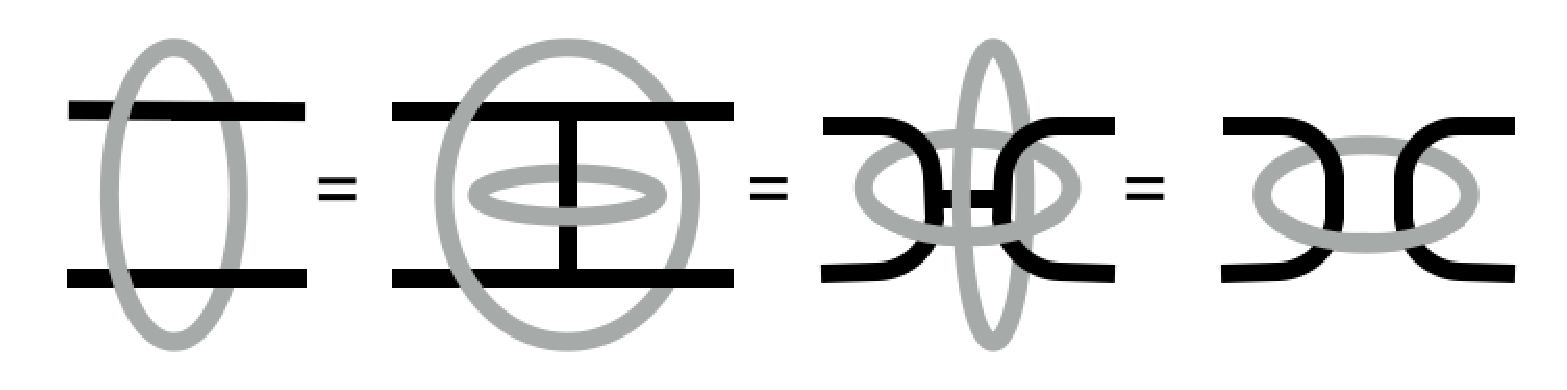
\includegraphics[width=120mm]{fig112.eps}
\end{center}
We can also easily confirm that the logical operators are invariant under this transformation as follows:
\begin{center}
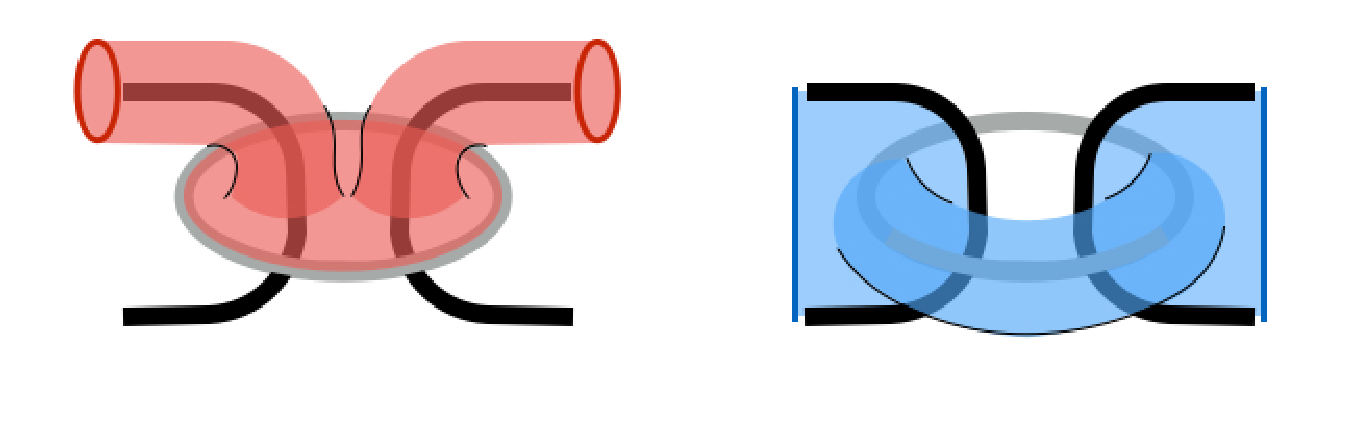
\includegraphics[width=120mm]{fig113.eps}
\end{center}

The $\Phi$-transformation is very useful to simplify a complicated topological operation on the surface by joining the tubes as follows:
\begin{center}
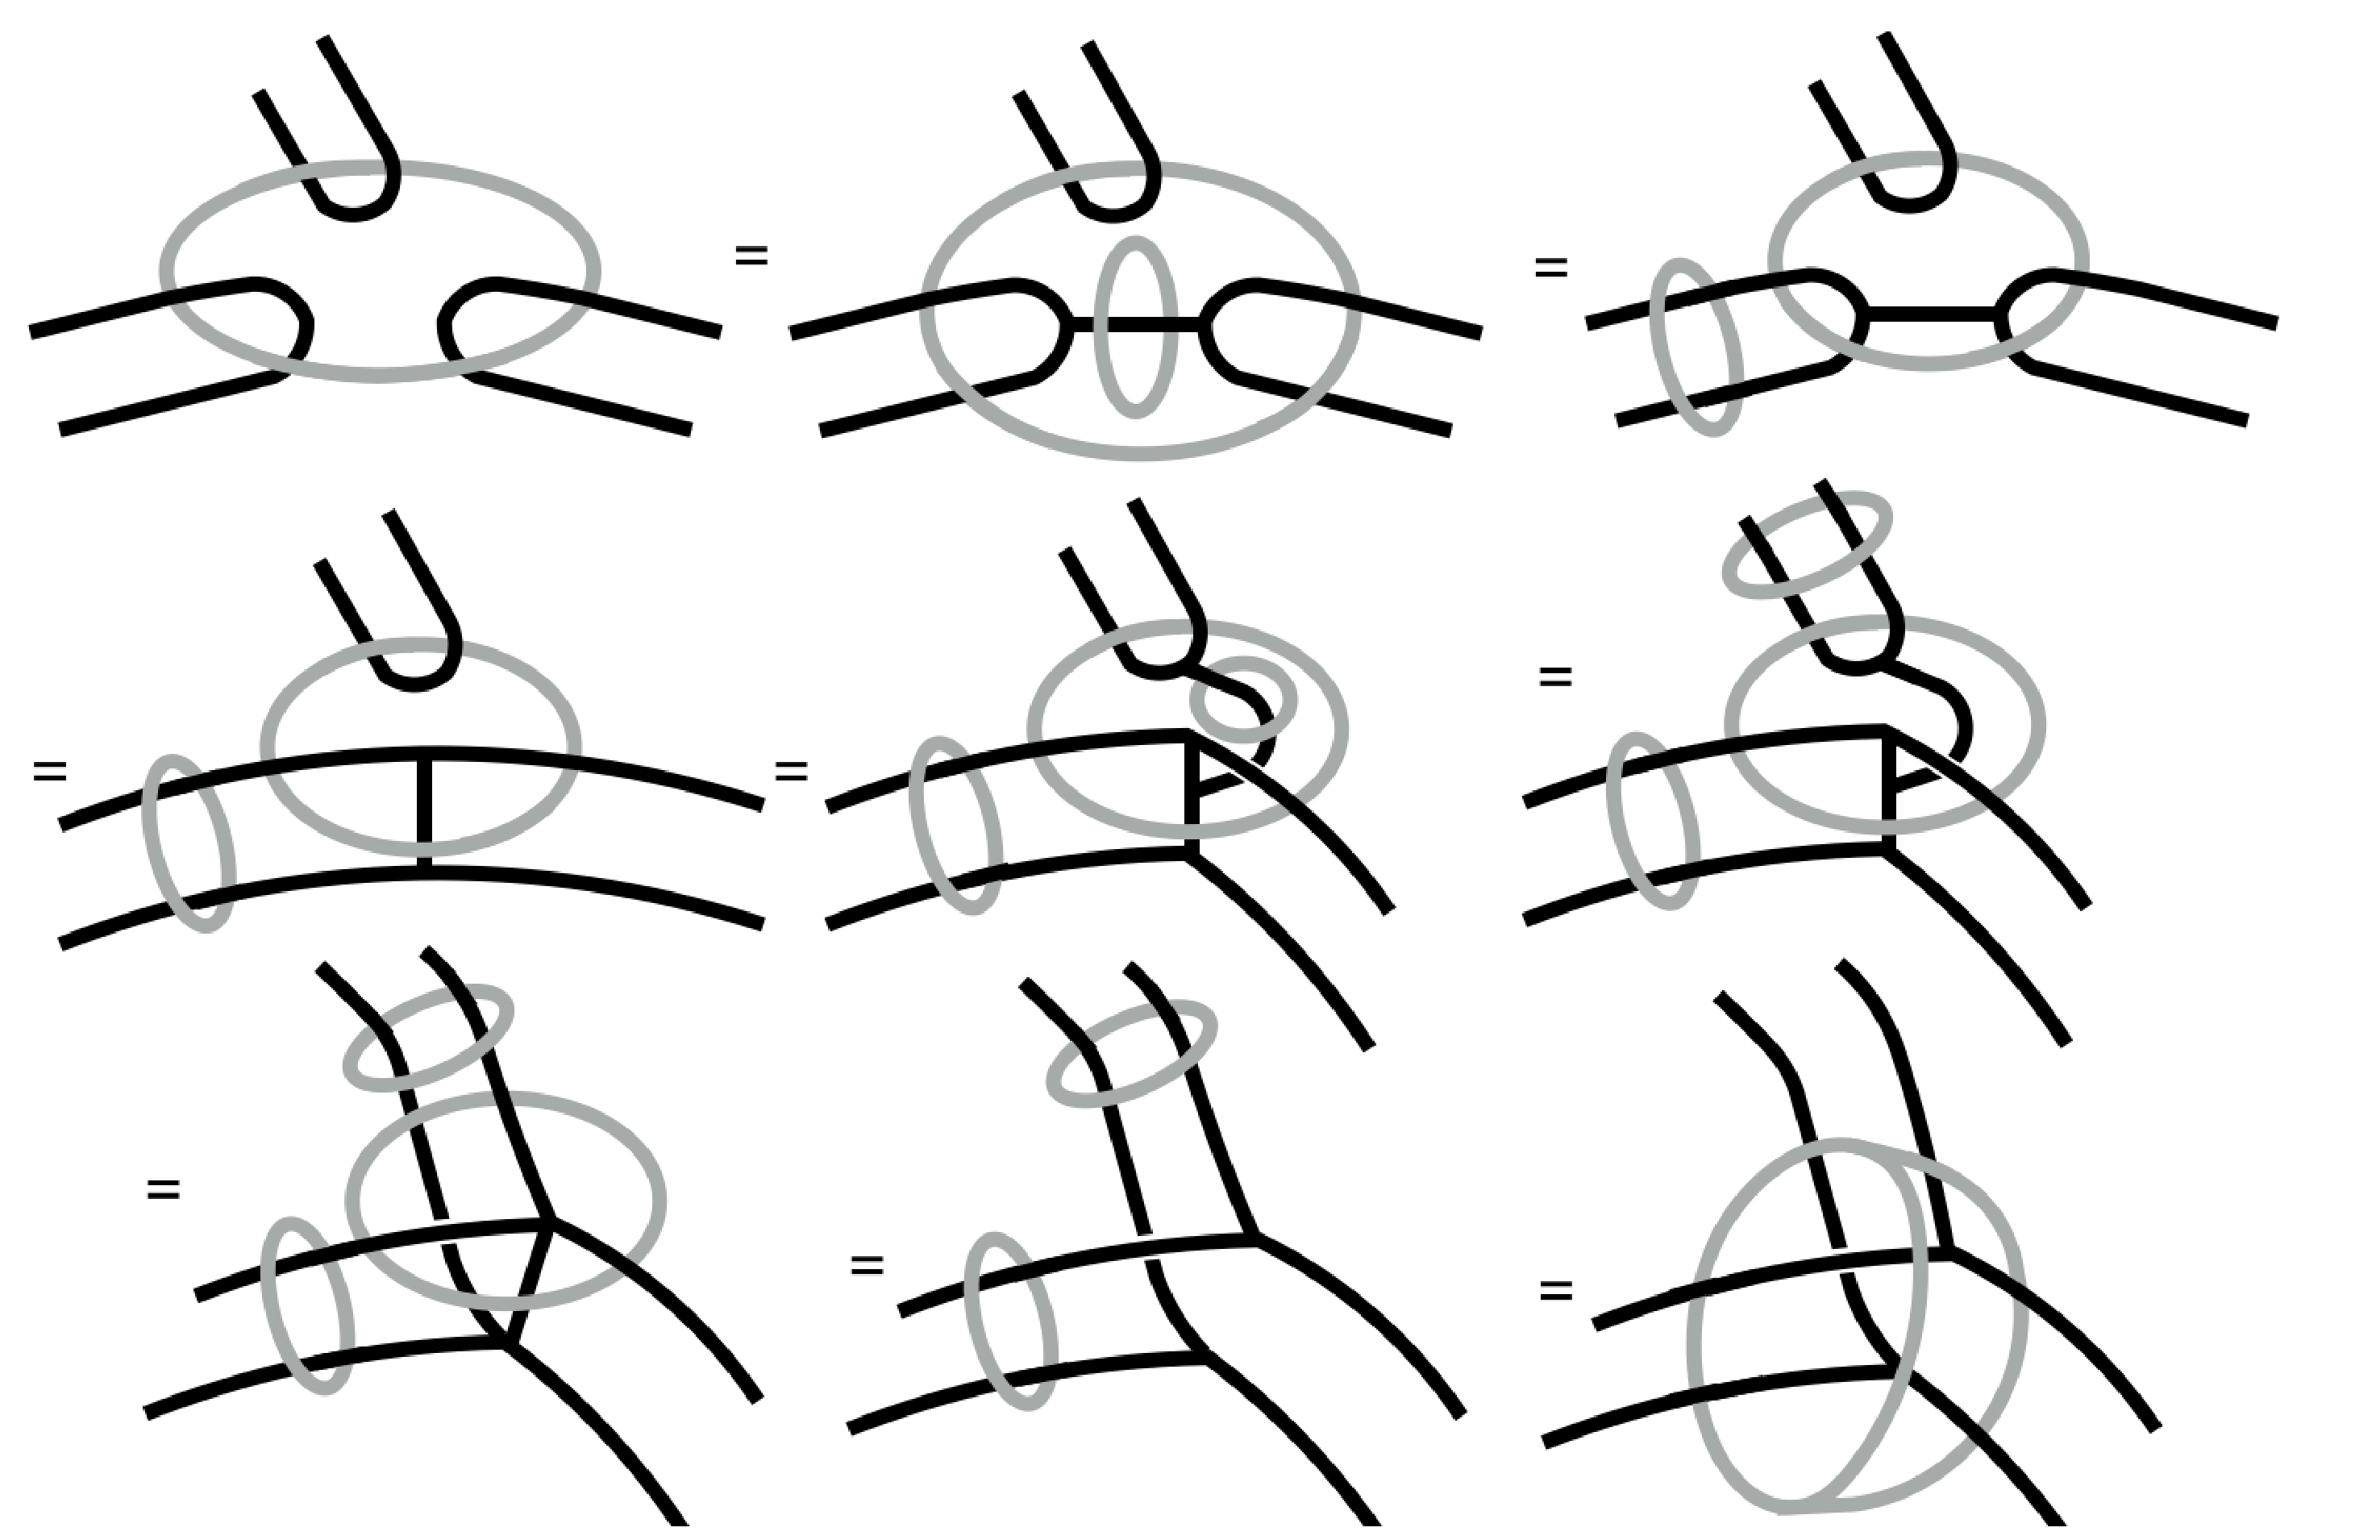
\includegraphics[width=140mm]{fig114.eps}
\end{center}
where we frequently used the $\Phi$-transformation and rule (\ref{TopoRule2}).
Here, the dual triple-ring wrapping around each of the two defect tubes serves to reflect the logical $Z$ operator from the upper to the lower tubes as follows:
\begin{center}
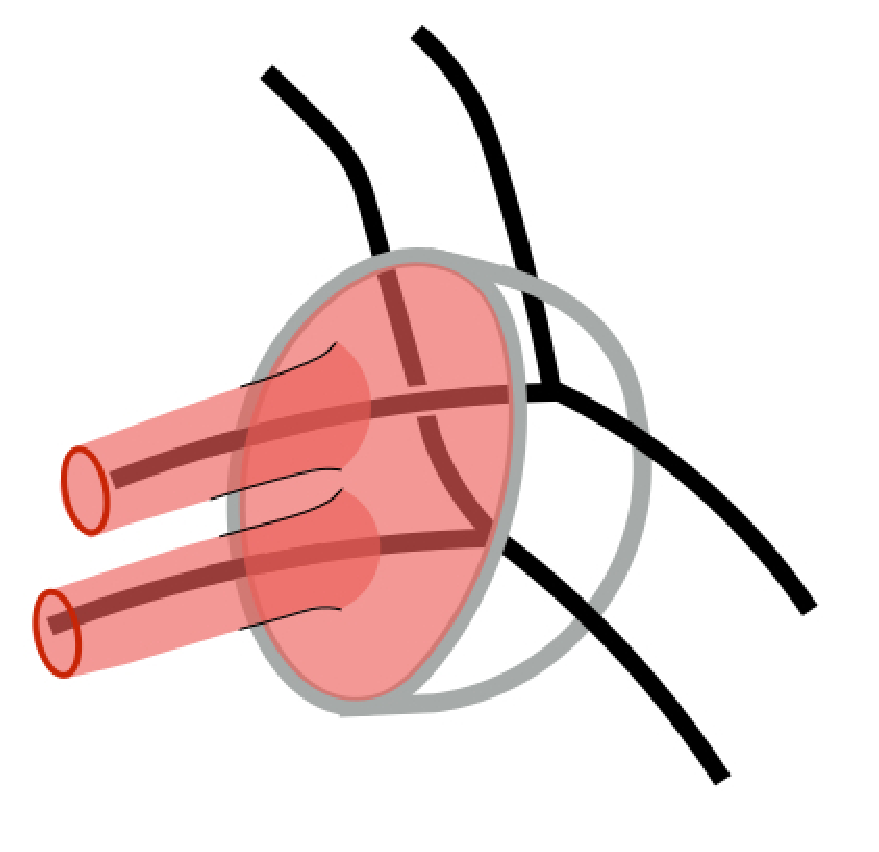
\includegraphics[width=50mm]{fig115.eps}
\end{center}

For example, if we apply this transformation to the CNOT gate between the primal defect pair qubits, we obtain a much simpler diagram as follows:
\begin{center}
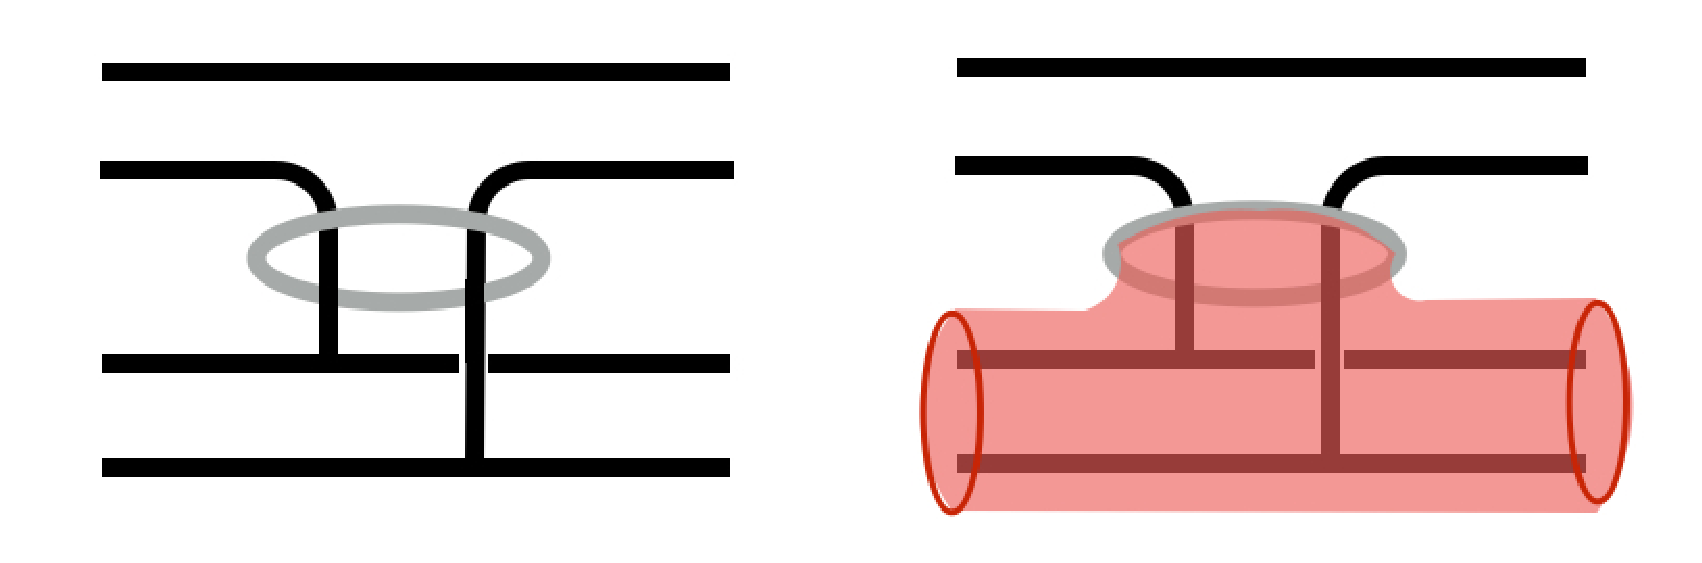
\includegraphics[width=100mm]{fig116.eps}
\end{center}
where the dual ring in the middle serves to keep the code space of the defect pair qubit as shown in the left above.
It is straightforward to check the transformations of the logical operators.
In general, by joining the defect tubes directly, we can transform the logical operators under multiple CNOT gates. 
However, if two tubes are joined, the definition of the defect pair is broken. 
In order to keep the defect pair qubit encoding, we need the dual ring wrapping around the two tubes at the joint.

The magic state injection is denoted by the following diagram:
\begin{center}
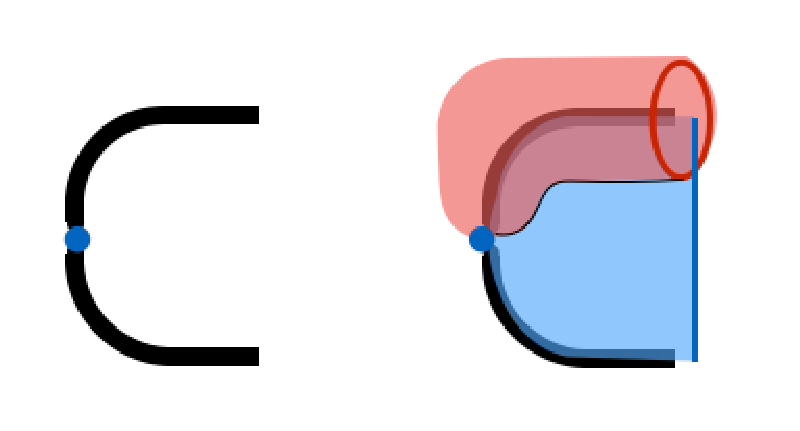
\includegraphics[width=80mm]{fig118.eps}
\end{center}
which can be viewed as a superposition of two correlation surfaces for the two anti-commuting logical operators.
The non-Clifford gate by one-bit teleportation can be described in the topological diagram as follows:
\begin{center}
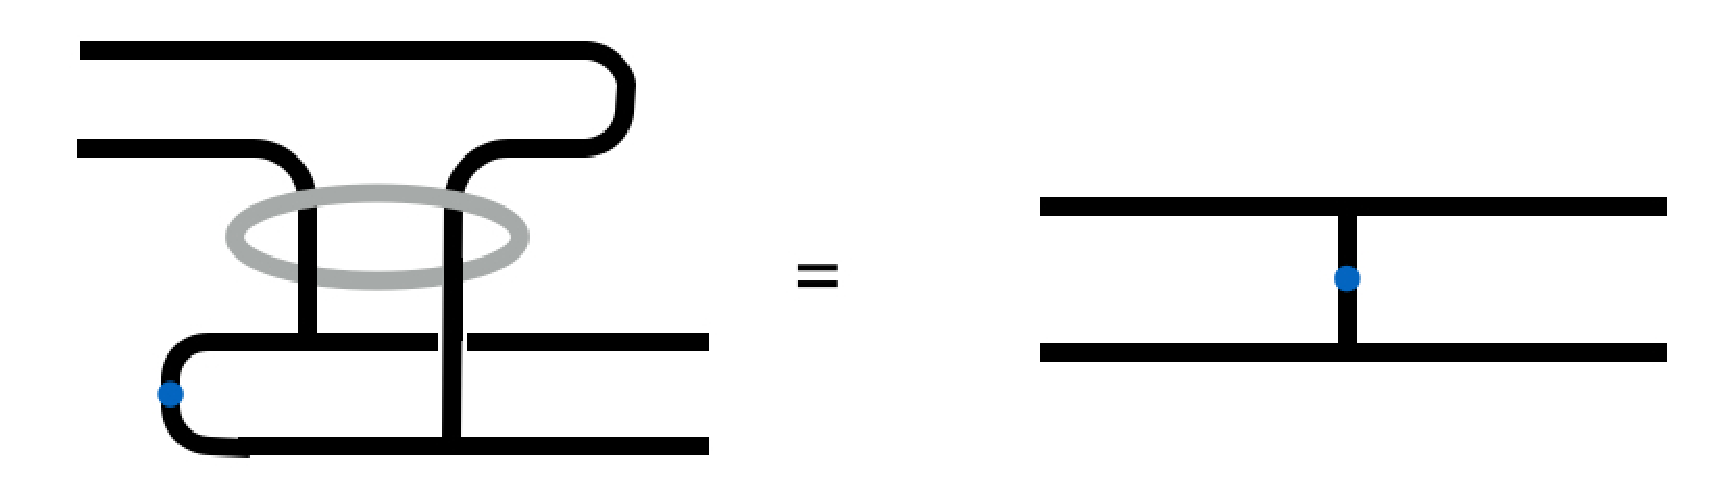
\includegraphics[width=100mm]{fig117.eps}
\end{center}
The right diagram, which is topologically equivalent to the left one, indicates that the non-Clifford gate by one-bit teleportation with the magic state injection is equivalent to simply performing the non-Clifford gate by the method mentioned in the previous section.

The present diagrammatic description of the topological operations and correlation surfaces on them provide us an intuitive understanding of how topological quantum computation on the surface code is performed.
These transformation rules will be useful to optimize the complexity (space-time volume required) of the braiding operations.

\section{Faulty syndrome measurements and noise thresholds}
\label{Sec:TopoFaultTolerance}
We have seen how universal quantum computation is executed on the surface code.
At each step, we have to perform topological quantum error correction to protect the quantum information encoded by the defects.
\begin{figure}[t]
\centering
%\sidecaption
% Use the relevant command for your figure-insertion program
% to insert the figure file.
% For example, with the option graphics use
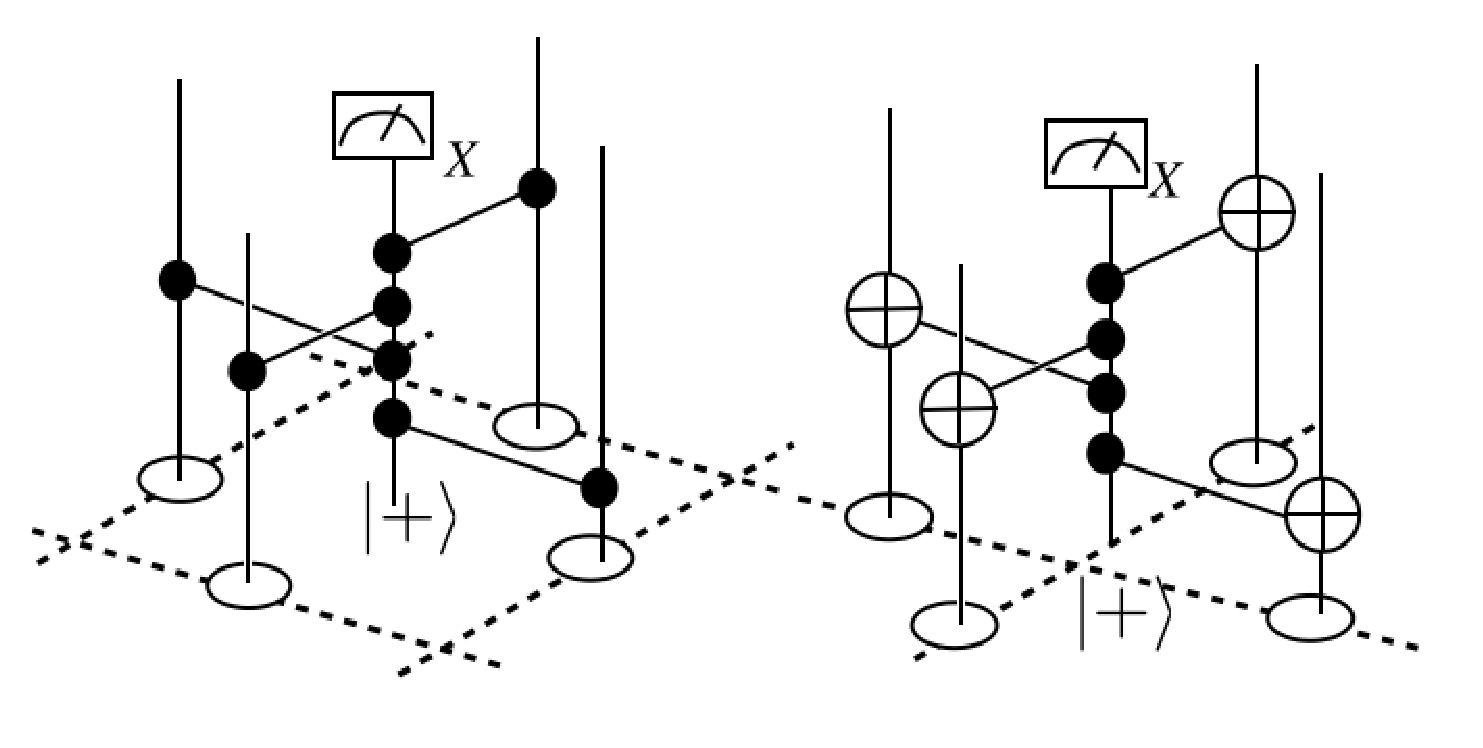
\includegraphics[width=120mm]{fig83.eps}
%
% If not, use
%\picplace{5cm}{2cm} % Give the correct figure height and width in cm
%
\caption{Syndrome measurements for plaquette (left) and star (right) operators, where qubits on a face center and on a vertex are employed as ancillae.
The alternative syndrome measurements for the plaquette and star operators are done repeatedly.}
\label{fig83}       % Give a unique label
\end{figure}
In Sec.~\ref{Sec:TQEC}, we analyzed topological quantum error correction on the surface code.
However, at that time, we assumed ideal syndrome measurements.
However, in a fault-tolerant quantum computation, we have to take into account all reasonable sources of noise, including faulty syndrome measurements, and the quantum computation has to tolerate them as well.
Here, we explain how faulty syndrome measurements are handled during topological quantum computation, which completes the big picture of fault-tolerant topological quantum computation.

During the topological operations, the star and plaquette operators are measured in the vacuum region to obtain the error syndrome.
These measurements are implemented using ancillae located on each vertex and face center for the star and plaquette operators, respectively (see Fig.~\ref{fig83}).
The ancilla state is prepared to be $|+\rangle$ and the $\Lambda (X)$ or $\Lambda(Z)$ gates are performed from the ancilla qubit as a control to the four qubits on $\partial f_l$ or $\delta v_k$.
By measuring the ancilla qubit in the $X$-basis, we obtain the eigenvalue of the star or plaquette operator. 
If an error is introduced during the measurement, we obtain an incorrect syndrome value, which has to be dealt with in the topological quantum error correction.

Again, we assume that the error is given as a Pauli error for simplicity.
We also assume that the $X$ and $Z$ errors, which might be correlated in general, are corrected independently.
The former assumption could be justified as follows.
Any Kraus operator of the noise map can be decomposed into a superposition of Pauli operators. 
Such a superposition is collapsed into Pauli errors by the syndrome measurements, which map different Pauli errors (of low weight) into orthogonal subspaces.
Note that, in this case, we have to model the error per gate carefully. 
The latter assumption makes the analysis very simple, but only results in an underestimation of the noise threshold.
Below we only consider correction of the $Z$ errors, but it can be applied straightforwardly to the $X$ errors.


Let $c_1^{e}(t) = \sum _l z^e_l(t) e_l$ be a 1-chain specifying the space-time $Z$ error location, where if $z_l(t)=1$, an $Z$ error occurs on qubit $e_l$ at time step $t$.  
The $Z$ operators on the code state at time $t$ are denoted by $c_1(t) = \sum _l z_l(t)$ (i.e., $Z[c_1(t)]$).%, which we call the state at time $t$.
 The state at time $t$ satisfies the following equation of the motion:
\begin{eqnarray}
c_1(t+1) = c_1(t) + c_1^{e} (t+1).
\end{eqnarray}
At each time step $t$, we measure the star operator $B_k(t)$ and obtain the measurement outcome
\begin{eqnarray}
m_k (t) = \left( \bigoplus _{e_l \in \delta v_k} z_l (t)  \right) \oplus z^e_k (t),
\end{eqnarray}
where the bit $z^e_k (t) \in \{ 0,1\}$ indicates an error on the measured syndrome, which we call a measurement error.
To obtain an equation consisting only of errors, we calculate the parity of the syndrome at time steps $t$ and $t-1$,
\begin{eqnarray}
s_k(t) = m_k (t) \oplus m_k(t-1) = \left( \bigoplus _{e_l \in \delta v_k} z^e_l (t) \right) \oplus z^e_k (t) \oplus z^e_k (t-1). 
\end{eqnarray}
Hence, errors on the measured syndrome can be detected by the parity (difference) of the syndrome values at time $t$ and $t-1$.
We redefine $\{ s_k (t) \}$ as an error syndrome of the space-time errors including the measurement error.
\begin{figure}[t]
\centering
%\sidecaption
% Use the relevant command for your figure-insertion program
% to insert the figure file.
% For example, with the option graphics use
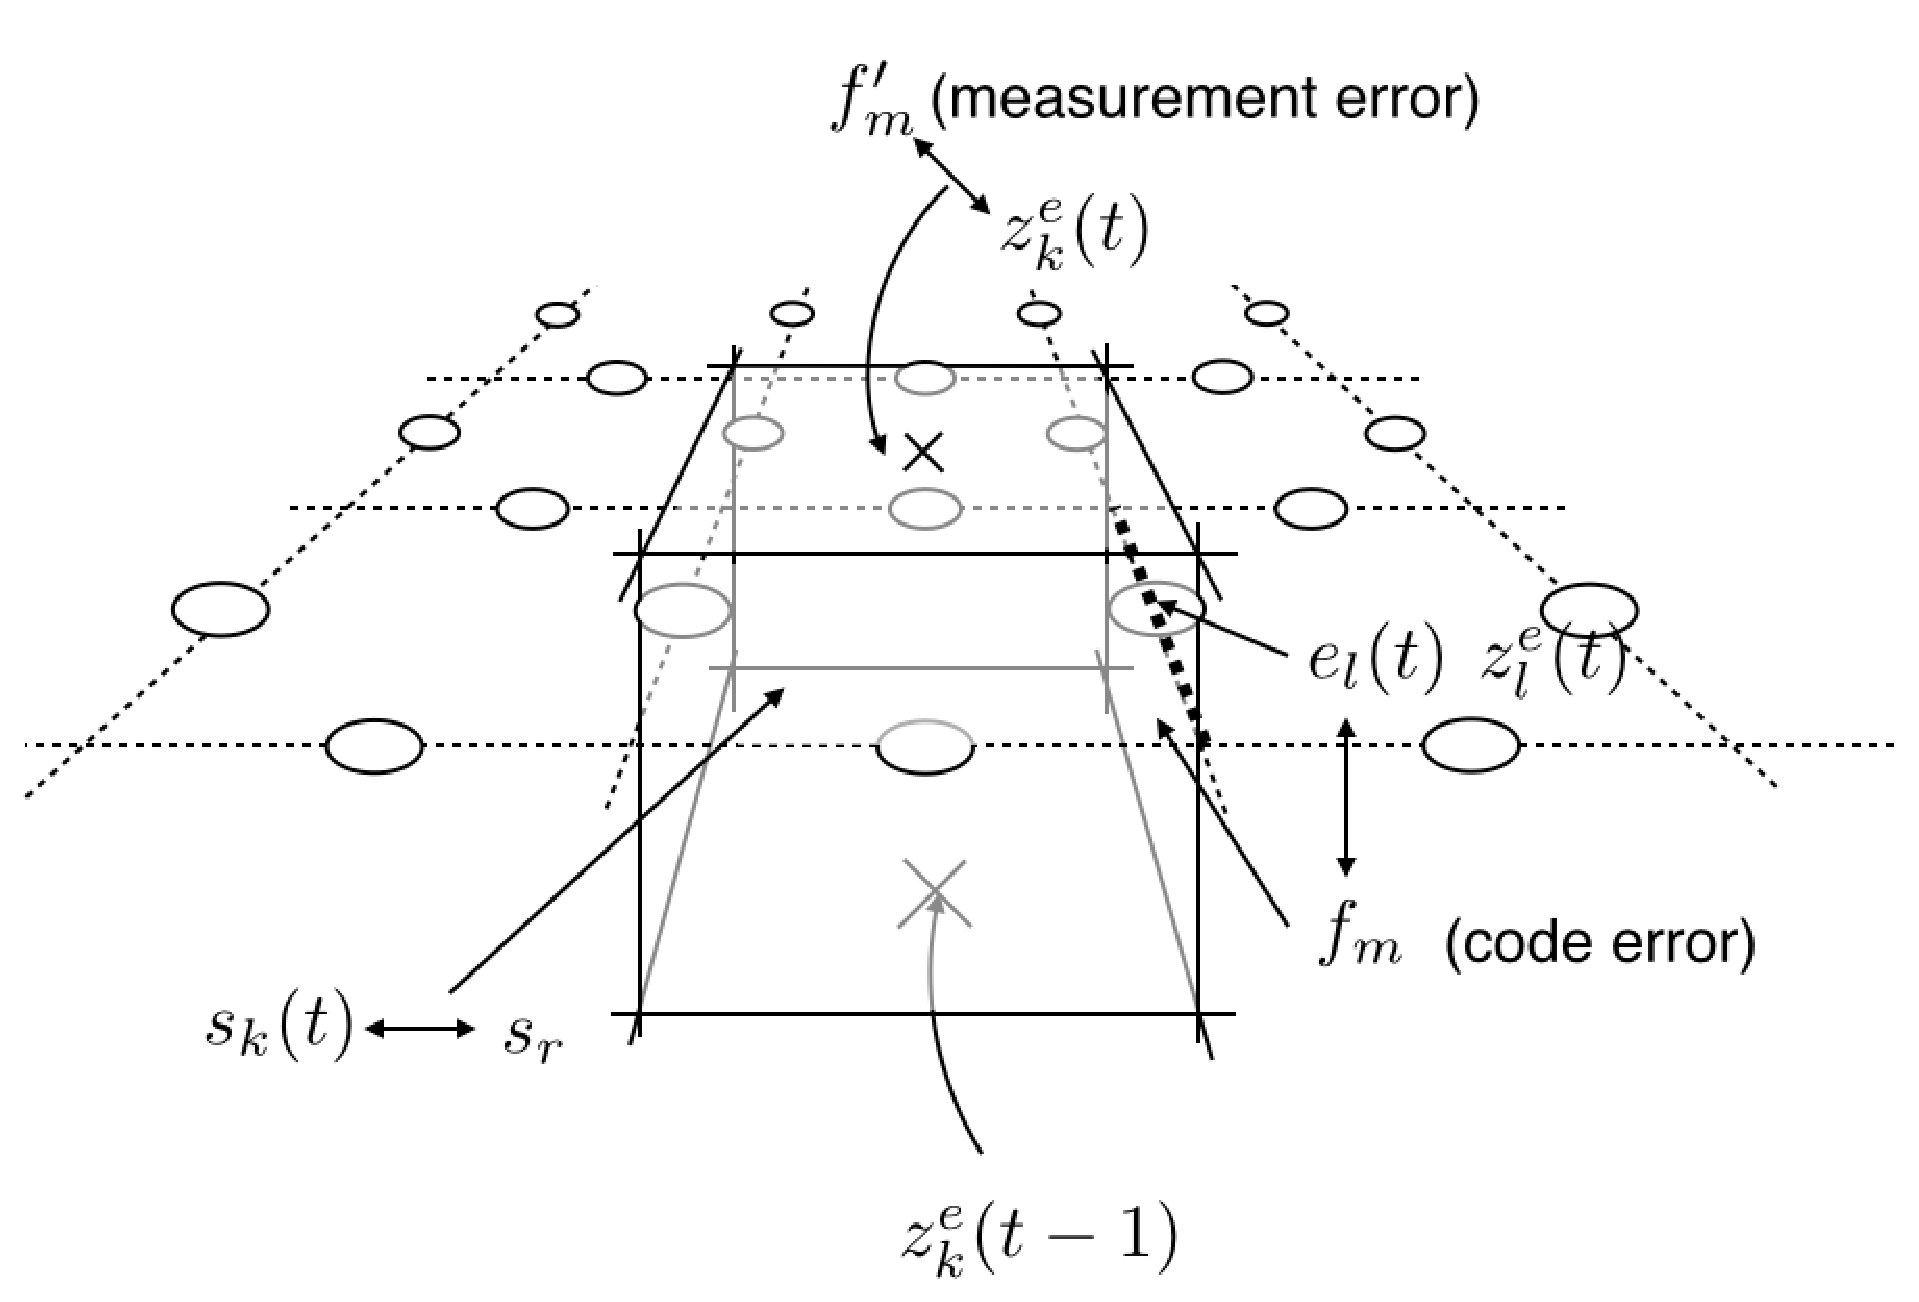
\includegraphics[width=130mm]{fig84.eps}
%
% If not, use
%\picplace{5cm}{2cm} % Give the correct figure height and width in cm
%
\caption{A mapping from the chain complex in 2D with time evolution to another chain complex in 3D.}
\label{fig84}       % Give a unique label
\end{figure}

In the case of the perfect syndrome measurement, the error syndrome is given by the boundary of errors $\partial c_1^e$, which allows us to use the MWPM algorithm for the error correction.
What about the case with the faulty syndrome measurement?
Using a chain complex in a 3D manifold, we can again reformulate the error syndrome $\{ s_k (t) \}$ as the boundary of a space-time error chain as shown in Fig.~\ref{fig84}.
We consider a chain complex $\{ C_0, C_1, C_2, C_3\}$ on a cubic lattice.
The basis for the 3-chain is given by a set of cubes $\{ q_r \}$. 
The 3-chain $c_3 = \sum _r z_r q_r \in C_3$ ($z_r\in \{ 0,1\}$) is a linear combination over $\mathbf{Z}_2$.
The dual chain complex $\{ \bar C_0, \bar C_1 , \bar C_2 , \bar C_3\}$ is also defined.
Specifically, $C_i$ and $C_{3-i}$ are identified via the duality transformation.

Let us explain how to embed the space-time error location to a 1-chain in the chain complex in 3D.
The edge $e_l(t)$ and its coefficient $z_l^e(t)$ at time $t$ are mapped into a vertical face $f_m$ and its coefficient $z_m^e$ in the 3D chain complex,
respectively.
The measurement error $z^e(t)$ is mapped to the coefficient $z_{m'}^e$ of a horizontal face $f_{m'}$.
Then, the space-time error location including the measurement errors is described by a 2-chain or a dual 1-chain in the 3D chain complex:
\begin{eqnarray}
c_2 ^e = \sum _m z_m^e f_m, \;\; \leftrightarrow \;\; \bar c_1 ^e = \sum _m z_m^e \bar e_m.
\end{eqnarray}
A syndrome $s_k (t)$ is assigned on each cube $q_r$, or equivalently each dual vertex $\bar v_ r$, in the 3D chain complex, and denoted by $s_r$.
Now we realize that 
\begin{eqnarray}
s_r = \bigoplus _{f_m \in q_r} z_m^e.
\end{eqnarray}
By using the same argument for the 2D case, $s_r =1$ iff $\bar v_r$ belongs to the boundary $\partial \bar c_1^e$ of the dual 1-chain $\bar c_1^e$, specifying the space-time error location.
Thus, we can apply the MWPM algorithm on the cubic lattice to perform topological quantum error correction in space-time. 

To calculate the noise thresholds, we have to model the noise distribution $P(\bar c_1^e)$.
First, we consider the simplest case, where the errors are located on each dual edge $\bar e_l$ of the dual cubic lattice with probability $p$.
This means that $Z$ errors occur on each qubit independently with probability $p$
at each time step.
Moreover, the measured syndrome is flipped with probability $p$.
Such a noise model is called a {\it phenomenological noise model}.
Using the MWPM algorithm, the noise threshold has been estimated to be $2.93\%$~\cite{Wang}.
The error correction problem under the phenomenological noise model can be mapped into a phase transition of the random-plaquette $\mathbf{Z}_2$ gauge model by using the same argument as in Sec.~\ref{Sec:TQECandSpinGlass}.
Specifically, the loop condition for the dual 1-chain (primal 2-chain) in the 3D model can be solved by introducing a gauge spin on each primal edge $\sigma _l$
and defining the dual trivial 1-cycle
$\bar c_1 = \sum _{m} z_m \bar e_m \in {\rm Img}(\bar \partial _2)$
via $(-1)^{z_m} = \prod _{e_l \in \partial f_m} \sigma _l$,
where $\bar e_m$ and $f_m$ are related through the duality relation.
In this way,
the variable on the face center
is provided as a product of the gauge spins on the boundary of the face, which leads to the random-plaquette $\mathbf{Z}_2$ gauge model.
The ordered Higgs and disordered confinement phases correspond to fault-tolerant and non-fault-tolerant regions, respectively~\cite{Dennis}.
The threshold value $2.93\%$ corresponds to the critical point at zero temperature.
The optimal threshold is provided on the Nishimori line and has been estimated to be $3.3\%$ using the Monte Carlo simulation~\cite{Ohno}.

In fault-tolerant quantum computation, we have to consider any source of noise, including the gate operations, during the syndrome measurement. 
As a standard way to model a realistic situation,
suppose that each elementary gate is followed by a depolarizing channel.
This is called a {\it circuit-based noise model}.
More precisely, 
an ideal single-qubit gate is followed by single-qubit depolarizing noise,
\begin{eqnarray}
(1-p_1)\rho + \sum _{A \in \{X,Y,Z\} } \frac{p_1}{3} A \rho  A.
\end{eqnarray}
An ideal two-qubit gate is followed by two-qubit depolarizing noise,
\begin{eqnarray}
(1-p_2)\rho + \sum _{A,B \in \{I, X,Y,Z\} \backslash I\otimes I} \frac{p_2}{15} (A\otimes B) \rho   (A\otimes B).
\end{eqnarray}
A faulty Pauli-basis state preparation is modeled by the state
\begin{eqnarray}
P_A^{+}(p_p) = (1-p_p) \frac{I+A}{2} + p_p \frac{I-A}{2},
\end{eqnarray}
where $A=X,Y,Z$.
A faulty Pauli-basis measurement is modeled by a POVM measurement with POVM elements
\begin{eqnarray}
\{ P_A^{+}(p_m), P_A^{-}(p_m)\},
\end{eqnarray}
where 
\begin{eqnarray}
P_A^{-}(p_m)= (1-p_m) \frac{I-A}{2} + p_m \frac{I+A}{2}.
\end{eqnarray}
Thus, the measurement outcome is flipped with probability $p_m$.

In Refs.~\cite{RaussendorfAnn,RaussendorfNJP,RaussendorfPRL}, the error probabilities were parameterized as $p_1 = p_2 = (3/2)p_p= (3/2)p_m$.
The noise threshold with the MWPM algorithm was obtained by numerical simulations to be $p_2 = 0.75\%$.
In Ref.~\cite{WangFowler}, the threshold value was further improved to $\sim 1\%$ by assigning a weight for each edge in MWPM appropriately, according to the amount of possible errors.
Roughly speaking, the threshold is located where the expectation value of each syndrome becomes $0.7$:
\begin{eqnarray}
\langle (-1)^{s_r} \rangle = 0.7.
\end{eqnarray}
In the phenomenological noise model, the expectation value is provided by
\begin{eqnarray}
\langle (-1)^{s_r} \rangle = (1-2p)^6,
\end{eqnarray}
which hits $0.7$ for $p=2.89\%$; thus being in good agreement with $2.93\%$.
Moreover, in the case of the circuit-based noise model, $p$ is roughly given by $p_p+p_m+4p_2$ for the measurement error, which means that one state preparation, one measurement, and four two-qubit gates are employed.
The error probability $p$ for the code state is given by $4p_2$, meaning that four two-qubit gates are employed in the syndrome measurements of the star and plaquette operators.
This yields
\begin{eqnarray}
\langle (-1)^{s_r} \rangle = (1-2p_p-2p_m-8p_2)^2 (1-8p_2)^4,
\end{eqnarray}
which hits 0.70 for $p_2 = 0.63\%$ with $p_1 = p_2 = (3/2)p_p= (3/2)p_m$.
This is again in a good agreement with the numerical result $0.75\%$.
This simple calculation provides rough estimates of the threshold values, but there is no validity.
If we need a more accurate threshold value, we should perform a numerical simulation by taking noise propagation and correlation into account~\cite{RaussendorfNJP,WangFowler}.


\section{Experimental progress}
Topologically protected quantum computation in 2D has been utilized as a platform to design fault-tolerant architectures for quantum computation.
One promising approach is on-chip monolithic architectures, such as quantum dots \cite{VanMeter,Jones12}, silicon-based nuclear spins~\cite{SiliconSpin}, and superconducting qubits \cite{Fowler1,Fowler2,IBM13,IBM14}, where huge number of qubits are integrated on a single chip and each individual qubit and the interactions between the qubits are manipulated by multiple lasers or electrodes.
Among them, the superconducting qubits system is one of the most promising candidates for implementing topological quantum computation on the surface code, because they can be fabricated on a 2D chip, and all elementary operations have already been demonstrated experimentally~\cite{ChargeQubit,ChargeCNOT,FluxQubit,DispersiveMeas}.
The coherence time and gate fidelity of the superconducting systems have improved rapidly.
An important breakthrough was made by Martinis's group at University of California Santa Barbara in 2014, where single-qubit gates with a fidelity of $99.92\%$ and two-qubit gates with a fidelity of $99.4\%$ were demonstrated on a 1D array of five superconducting transmon qubits~\cite{MartinisLegend,QuantumQuest}.
In addition, repetitive quantum non-demolition measurements were demonstrated on a 1D array of 9 qubits, which improved the fidelity of a state preparation by a factor of 8.5, even when using 9 qubits and faulty two-qubit gates and measurements~\cite{Martinis9qubit}.
This is an important building block of the fault-tolerant quantum computation on the surface code.

Another approach is the distributed modular architecture, where few-qubit local modules are connected with quantum channels mediating interactions between separate modules~\cite{LiBenjamin,FTProb,FujiiDis,Benjamin1,Benjamin2,Monroe}.
The few-qubit quantum module has already been experimentally realized in various physical systems, such as nitrogen-vacancy centers in diamond and trapped ions.
Furthermore, entangling operations between separate local modules have been experimentally demonstrated.
This experimental and theoretical progress will gradually lead us to large-scale quantum computation.